% chapters/ch01.tex
% 第~
% \ref{chap:1}~章 Hahn--Banach 定理. 共轭凸函数理论引论
% 源: 原书 PDF 第 12--40 页 (印刷页 1--29)

\chapter{Hahn--Banach 定理. 共轭凸函数理论引论}
\label{chap:1}

\index{bansuisuanzi@伴随算子 (adjoint)}
\index{Hahn--Banach theorem@Hahn--Banach 定理 (Hahn--Banach theorem)}
\section{Hahn--Banach 定理的解析形式: 线性泛函的延拓}
\label{sec:1.1}

设 $E$ 为 $\R$ 上的向量空间. 回忆\emph{泛函}是指定义在 $E$ 上 (或 $E$ 的某个子空间上),
取值于 $\R$ 的函数. 本节的主要结果, 是关于把定义在 $E$ 的线性子空间上的线性泛函
延拓为定义在整个 $E$ 上的线性泛函.

\index{HahnBanachdingli@Hahn--Banach 定理!jiexixingshi@解析形式 (Hahn--Banach theorem, analytic form)}
\index{Helly@Helly (Helly)}
\begin{theorem}[Helly, Hahn--Banach 解析形式]
\label{thm:1.1}
设 $p:E\to\R$ 为满足\footnote{满足 \eqref{eq:1.1} 与 \eqref{eq:1.2} 的函数 $p$ 有时称为
\emph{\index{Minkowskifanhan@Minkowski 泛函 (Minkowski functional)}
Minkowski 泛函}(Minkowski functional).}
\begin{align}
p(\lambda x) &= \lambda p(x) && \forall x\in E \quad\text{及}\quad \forall\lambda>0,
  \label{eq:1.1}\\
p(x+y) &\le p(x)+p(y) && \forall x,y\in E
  \label{eq:1.2}
\end{align}
的函数.设 $G\subset E$ 为线性子空间, $g:G\to\R$ 为满足
\begin{equation}
g(x)\le p(x)\quad \forall x\in G
  \label{eq:1.3}
\end{equation}
的线性泛函.在这些假设下, 存在定义在整个 $E$ 上的线性泛函 $f$, 它延拓 $g$, 即
$g(x)=f(x)\ \forall x\in G$, 并且满足
\begin{equation}
f(x)\le p(x)\quad \forall x\in E.
  \label{eq:1.4}
\end{equation}
\end{theorem}

定理  \ref{thm:1.1} 的证明依赖于 \index{Zornyinli@Zorn 引理 (Zorn's lemma)}
Zorn 引理, 这是关于有序集的一条著名而非常有用的性质.
在叙述 Zorn 引理之前, 我们须澄清一些概念.设 $P$ 为带 (偏) 序关系 $\le$ 的集合.
若对 $Q$ 中任意一对 $(a,b)$, 或者 $a\le b$, 或者 $b\le a$ (或二者兼有!), 则称子集 $Q\subset P$
为\emph{全序}的.设 $Q\subset P$ 为 $P$ 的子集; 若对每个 $a\in Q$ 都有 $a\le c$, 则称 $c\in P$
为 $Q$ 的\emph{上界}.若不存在 $x\in P$ 使得 $m\le x$ (除非 $x=m$), 则称 $m\in P$ 为 $P$ 的
\emph{极大元}.注意 $P$ 的极大元不必是 $P$ 的上界.

若 $P$ 中每个全序子集 $Q$ 都有上界, 则称 $P$ 是\emph{归纳的}.

\begin{keylemma}[Zorn]
\label{lem:1.1}
每个非空且归纳的有序集都有极大元.
\end{keylemma}

Zorn 引理可由选择公理推出, 但我们在此不讨论它的推导; 可参见例如 J.~Dugundji
\bref{Dugundji}{1}, N.~Dunford--J.~T.~Schwartz \bref{DunfordSchwartz}{1} (第 1 卷,
定理 1.2.7), E.~Hewitt--K.~Stromberg \bref{HewittStromberg}{1}, S.~Lang \bref{Lang}{1}
以及 A.~Knapp \bref{Knapp}{1}.

\begin{remark}
\label{rem:1.1}
Zorn 引理在分析中有许多重要的应用.它是在证明某些看似天真的存在性命题时的基本工具,
例如``每个向量空间都有基''(见习题  \ref{exer:1.5}) 和``任何向量空间上都存在非平凡的
线性泛函''.多数分析学家并不知道如何证明 Zorn 引理; 但对分析学家而言,
理解 Zorn 引理的陈述并能够正确地使用它, 却是相当要紧的!
\end{remark}

\begin{proof}[引理 \ref{lem:1.2}]
% 原书此处误作 "Proof of Lemma 1.2", 实际证明的是定理 1.1 (真正的引理~
% \ref{lem:1.2} 的证明见
% 印刷页 6). 两份 OCR 与 PDF 文本层一致, 属原书排印之误. 依技能规范: 保留原样并记录,
% 不擅自更正. 见《项目交接文档》"原书疑似错误"条目.
考虑集合
\begin{equation*}
P=\left\{h:D(h)\subset E\to\R\ \middle|\
\begin{array}{l}
D(h)\ \text{是}\ E\ \text{的线性子空间},\\
h\ \text{线性},\quad G\subset D(h),\\
h\ \text{延拓}\ g,\ \text{且}\ h(x)\le p(x)\quad\forall x\in D(h)
\end{array}
\right\}.
\end{equation*}
在 $P$ 上定义序关系
\begin{equation*}
(h_1\le h_2)\iff\bigl(D(h_1)\subset D(h_2)\ \text{且}\ h_2\ \text{延拓}\ h_1\bigr).
\end{equation*}
显然 $P$ 非空, 因为 $g\in P$.我们断言 $P$ 是归纳的.事实上, 设 $Q\subset P$ 为全序子集;
把 $Q$ 写成 $Q=(h_i)_{i\in I}$, 并置
\begin{equation*}
D(h)=\bigcup_{i\in I}D(h_i),\qquad
h(x)=h_i(x)\quad \text{若}\ x\in D(h_i)\ \text{对某个}\ i.
\end{equation*}
容易看出 $h$ 的定义是有意义的, $h\in P$, 且 $h$ 是 $Q$ 的上界.于是我们可以应用 Zorn 引理,
从而得到 $P$ 中的一个极大元 $f$.我们断言 $D(f)=E$, 这就完成了定理  \ref{thm:1.1} 的证明.

反设 $D(f)\ne E$.取 $x_0\notin D(f)$; 置 $D(h)=D(f)+\R x_0$, 并对每个 $x\in D(f)$ 置
$h(x+tx_0)=f(x)+t\alpha\ (t\in\R)$, 其中常数 $\alpha\in\R$ 将被选得使 $h\in P$.
我们必须保证
\begin{equation*}
f(x)+t\alpha\le p(x+tx_0)\quad \forall x\in D(f)\quad\text{及}\quad \forall t\in\R.
\end{equation*}
由 \eqref{eq:1.1} 只需验证
\begin{equation*}
\begin{cases}
f(x)+\alpha\le p(x+x_0) & \forall x\in D(f),\\
f(x)-\alpha\le p(x-x_0) & \forall x\in D(f).
\end{cases}
\end{equation*}
换言之, 我们必须找到某个 $\alpha$ 满足
\begin{equation*}
\sup_{y\in D(f)}\{f(y)-p(y-x_0)\}\le\alpha\le
\inf_{x\in D(f)}\{p(x+x_0)-f(x)\}.
\end{equation*}
这样的 $\alpha$ 存在, 因为
\begin{equation*}
f(y)-p(y-x_0)\le p(x+x_0)-f(x)\quad \forall x\in D(f),\ \forall y\in D(f);
\end{equation*}
事实上, 由 \eqref{eq:1.2} 可得
\begin{equation*}
f(x)+f(y)\le p(x+y)\le p(x+x_0)+p(y-x_0).
\end{equation*}
于是 $f\le h$; 但这是不可能的, 因为 $f$ 是极大元且 $h\ne f$.
\end{proof}

现在描述定理  \ref{thm:1.1} 在 $E$ 为赋范向量空间 (n.v.s.), 范数为 $\norm{\cdot}$ 的情形下的
一些简单应用.

\begin{notation}
记 $E^\star$ 为 $E$ 的\emph{\index{duioukongjian@对偶空间 (dual space)}
对偶空间}, 即 $E$ 上一切连续线性泛函构成的空间;
$E^\star$ 上的 (对偶) 范数定义为
\begin{equation}
\norm{f}_{E^\star}=\sup_{\substack{x\in E\\ \norm{x}\le 1}}\abs{f(x)}
=\sup_{\substack{x\in E\\ \norm{x}\le 1}}f(x).
  \label{eq:1.5}
\end{equation}
在不致混淆时, 我们也用 $\norm{f}$ 代替 $\norm{f}_{E^\star}$.

给定 $f\in E^\star$ 与 $x\in E$, 我们常写 $\dual{f}{x}$ 代替 $f(x)$;
并称 $\dual{\cdot}{\cdot}$ 为对偶 $E^\star,E$ 的\emph{标量积}.

众所周知 $E^\star$ 是 Banach 空间, 即 $E^\star$ 是完备的 (即使 $E$ 不完备);
这可由 $\R$ 完备这一事实推出.
\end{notation}

\begin{keycorollary}
\label{cor:1.2}
设 $G\subset E$ 为线性子空间.若 $g:G\to\R$ 为连续线性泛函, 则存在 $f\in E^\star$
延拓 $g$, 且
\begin{equation*}
\norm{f}_{E^\star}=\sup_{\substack{x\in G\\ \norm{x}\le 1}}\abs{g(x)}=\norm{g}_{G^\star}.
\end{equation*}
\end{keycorollary}

\begin{proof}
在定理  \ref{thm:1.1} 中取 $p(x)=\norm{g}_{G^\star}\norm{x}$.
\end{proof}

\begin{keycorollary}
\label{cor:1.3}
对每个 $x_0\in E$ 都存在 $f_0\in E^\star$ 使得
\begin{equation*}
\norm{f_0}=\norm{x_0}\quad\text{且}\quad \dual{f_0}{x_0}=\norm{x_0}^2.
\end{equation*}
\end{keycorollary}

\begin{proof}
在推论  \ref{cor:1.2} 中取 $G=\R x_0$ 及 $g(tx_0)=t\norm{x_0}^2$, 于是
$\norm{g}_{G^\star}=\norm{x_0}$.
\end{proof}

\begin{remark}
\label{rem:1.2}
推论  \ref{cor:1.3} 给出的元素 $f_0$ 一般并不唯一 (试着构造一个例子, 或见习题
 \ref{exer:1.2}).然而, 若 $E^\star$ 是\index{yangetufanshu@严格凸范数 (strictly convex norm)}
严格凸的\footnote{若
$\norm{tx+(1-t)y}<1,\ \forall t\in(0,1),\ \forall x,y$ 满足 $\norm{x}=\norm{y}=1$ 且
$x\ne y$, 则称赋范空间是\emph{严格凸}的; 见习题  \ref{exer:1.26}.}
——例如 $E$ 为 Hilbert 空间 (见第~
\ref{chap:5}~章), 或 $E=L^p(\Omega)$ 且 $1<p<\infty$
(见第~
\ref{chap:4}~章)——则 $f_0$ 是唯一的.一般地, 我们对每个 $x_0\in E$ 置
\begin{equation*}
F(x_0)=\bigl\{f_0\in E^\star;\ \norm{f_0}=\norm{x_0}\ \text{且}\ \dual{f_0}{x_0}=\norm{x_0}^2\bigr\}.
\end{equation*}
这个 (多值的) 映射 $x_0\mapsto F(x_0)$ 称为从 $E$ 到 $E^\star$ 的\emph{\index{duiouyingshe@对偶映射 (duality map)}
对偶映射};
它的某些性质在习题  \ref{exer:1.1},  \ref{exer:1.2},  \ref{exer:3.28} 与问题 13 中有描述.
\end{remark}

\begin{keycorollary}
\label{cor:1.4}
对每个 $x\in E$ 都有
\begin{equation}
\norm{x}=\sup_{\substack{f\in E^\star\\ \norm{f}\le 1}}\abs{\dual{f}{x}}
=\max_{\substack{f\in E^\star\\ \norm{f}\le 1}}\abs{\dual{f}{x}}.
  \label{eq:1.6}
\end{equation}
\end{keycorollary}

\begin{proof}
我们总可假设 $x\ne 0$.显然
\begin{equation*}
\sup_{\substack{f\in E^\star\\ \norm{f}\le 1}}\abs{\dual{f}{x}}\le\norm{x}.
\end{equation*}
另一方面, 由推论  \ref{cor:1.3} 知存在 $f_0\in E^\star$ 使得 $\norm{f_0}=\norm{x}$ 且
$\dual{f_0}{x}=\norm{x}^2$.置 $f_1=f_0/\norm{x}$, 于是 $\norm{f_1}=1$ 且
$\dual{f_1}{x}=\norm{x}$.
\end{proof}

\begin{remark}
\label{rem:1.3}
公式 \eqref{eq:1.5}——它是一个\emph{定义}——不应与公式 \eqref{eq:1.6} 混淆,
后者是一个\emph{命题}.一般地, \eqref{eq:1.5} 中的 ``sup'' 未必取到; 例如见习题
 \ref{exer:1.3}.然而, 若 $E$ 是自反 Banach 空间 (见第~
\ref{chap:3}~章), 则 \eqref{eq:1.5} 中的
``sup'' 可以取到; R.~C.~James 的一个深刻结果断言其逆亦真: 若 $E$ 是 Banach 空间,
且对每个 $f\in E^\star$, \eqref{eq:1.5} 中的 sup 都能取到, 则 $E$ 自反; 参见例如
J.~Diestel \brefcite{Diestel}{1}{, 第 1 章} 或 R.~Holmes \bref{Holmes}{1}.
\end{remark}

\section{Hahn--Banach 定理的几何形式: 凸集的分离}
\label{sec:1.2}

我们先给出关于超平面的一些预备事实.以下 $E$ 均指赋范向量空间.

\begin{definition}
\emph{仿射超平面}是指 $E$ 的如下形式的子集
\begin{equation*}
H=\{x\in E;\ f(x)=\alpha\},
\end{equation*}
其中 $f$ 是不恒为零的线性泛函\footnote{我们不假定 $f$ 连续 (在每个无穷维赋范空间中都存在
不连续的线性泛函; 见习题  \ref{exer:1.5}).}, $\alpha\in\R$ 为给定常数.
我们写 $H=[f=\alpha]$, 并称 $f=\alpha$ 是 $H$ 的方程.
\end{definition}

\begin{proposition}
\label{prop:1.5}
超平面 $H=[f=\alpha]$ 是闭的, 当且仅当 $f$ 连续.
\end{proposition}

\begin{proof}
显然, 若 $f$ 连续则 $H$ 闭.反之, 设 $H$ 闭.$H$ 的补集 $H^c$ 是开的且非空
(因为 $f$ 不恒为零).取 $x_0\in H^c$, 于是 $f(x_0)\ne\alpha$, 例如 $f(x_0)<\alpha$.
取 $r>0$ 使得 $B(x_0,r)\subset H^c$, 其中
\begin{equation*}
B(x_0,r)=\{x\in E;\ \norm{x-x_0}<r\}.
\end{equation*}
我们断言
\begin{equation}
f(x)<\alpha\quad \forall x\in B(x_0,r).
  \label{eq:1.7}
\end{equation}
事实上, 反设对某个 $x_1\in B(x_0,r)$ 有 $f(x_1)>\alpha$.线段
\begin{equation*}
\{x_t=(1-t)x_0+tx_1;\ t\in[0,1]\}
\end{equation*}
包含在 $B(x_0,r)$ 中, 从而 $f(x_t)\ne\alpha,\ \forall t\in[0,1]$; 另一方面, 对某个
$t\in[0,1]$ 有 $f(x_t)=\alpha$, 即 $t=\dfrac{f(x_1)-\alpha}{f(x_1)-f(x_0)}$,
矛盾, 故 \eqref{eq:1.7} 得证.由 \eqref{eq:1.7} 推出
\begin{equation*}
f(x_0+rz)<\alpha\quad \forall z\in B(0,1).
\end{equation*}
因此 $f$ 连续, 且 $\norm{f}\le\dfrac{1}{r}\bigl(\alpha-f(x_0)\bigr)$.
\end{proof}

\begin{definition}
设 $A,B$ 为 $E$ 的两个子集.若
\begin{equation*}
f(x)\le\alpha\quad \forall x\in A\quad\text{且}\quad f(x)\ge\alpha\quad \forall x\in B,
\end{equation*}
则称超平面 $H=[f=\alpha]$ \emph{分离} $A$ 与 $B$.

若存在 $\varepsilon>0$ 使得
\begin{equation*}
f(x)\le\alpha-\varepsilon\ \ \forall x\in A\quad\text{且}\quad
f(x)\ge\alpha+\varepsilon\ \ \forall x\in B,
\end{equation*}
则称 $H$ \emph{严格分离} $A$ 与 $B$.

从几何上说, 分离意味着 $A$ 位于 $H$ 所决定的半空间之一中, 而 $B$ 位于另一个半空间中;
见图  \ref{fig:1}.

最后回忆, 子集 $A\subset E$ 称为\emph{凸}的, 若
\begin{equation*}
tx+(1-t)y\in A\quad \forall x,y\in A,\quad \forall t\in[0,1].
\end{equation*}
\end{definition}

\index{tujifenli@凸集分离 (separation of convex sets)}
\begin{keytheorem}[Hahn--Banach, 第一几何形式]
\label{thm:1.6}
设 $A\subset E$ 与 $B\subset E$ 为两个非空凸子集, 且 $A\cap B=\emptyset$.
假设其中一个是开的.则存在分离 $A$ 与 $B$ 的闭超平面.
\end{keytheorem}

定理  \ref{thm:1.6} 的证明依赖于下面两条引理.

\begin{figure}[htbp]
	\centering
	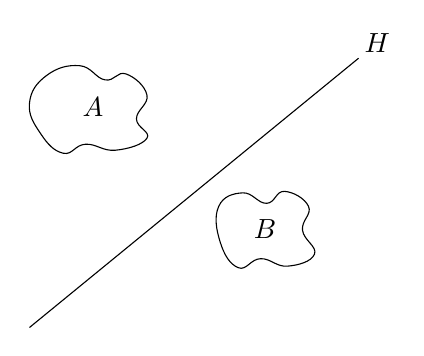
\begin{tikzpicture}[scale=0.95]
		% 超平面 H (斜线)
		\draw (0.2,-0.6) -- (4.6,3.0) node[above right, inner sep=2pt] {$H$};
		% 凸集 A (H 左上方)
		\begin{scope}[shift={(1.05,2.35)}]
			\draw plot[smooth cycle, tension=0.75] coordinates {
				(-0.85,0.05) (-0.62,0.42) (-0.18,0.55) (0.16,0.36)
				(0.44,0.44) (0.72,0.16) (0.58,-0.16) (0.72,-0.42)
				(0.30,-0.58) (-0.10,-0.50) (-0.40,-0.62) (-0.70,-0.36)};
		\end{scope}
		\node at (1.05,2.35) {$A$};
		% 凸集 B (H 右下方)
		\begin{scope}[shift={(3.35,0.72)}]
			\draw plot[smooth cycle, tension=0.75] coordinates {
				(-0.62,0.30) (-0.30,0.48) (0.02,0.34) (0.26,0.50)
				(0.58,0.30) (0.50,-0.02) (0.66,-0.34) (0.30,-0.50)
				(-0.06,-0.40) (-0.36,-0.52) (-0.60,-0.18)};
		\end{scope}
		\node at (3.35,0.72) {$B$};
	\end{tikzpicture}
	\caption{}
	\label{fig:1}
\end{figure}

\begin{lemma}
\label{lem:1.2}
设 $C\subset E$ 为含 $0\in C$ 的开凸集.对每个 $x\in E$ 置
\begin{equation}
p(x)=\inf\{\alpha>0;\ \alpha^{-1}x\in C\}
  \label{eq:1.8}
\end{equation}
($p$ 称为 $C$ 的\emph{规范函数}(gauge) 或 $C$ 的 Minkowski 泛函).
则 $p$ 满足 \eqref{eq:1.1}, \eqref{eq:1.2} 以及下述性质:
\begin{align}
&\text{存在常数 } M \text{ 使得}\quad 0\le p(x)\le M\norm{x}\quad \forall x\in E,
  \label{eq:1.9}\\
&C=\{x\in E;\ p(x)<1\}.
  \label{eq:1.10}
\end{align}
\end{lemma}

\begin{proof}
显然 \eqref{eq:1.1} 成立.

\emph{\eqref{eq:1.9} 的证明.} 取 $r>0$ 使得 $B(0,r)\subset C$; 显然有
\begin{equation*}
p(x)\le\frac{1}{r}\norm{x}\quad \forall x\in E.
\end{equation*}

\emph{\eqref{eq:1.10} 的证明.} 先设 $x\in C$; 因 $C$ 开, 故当 $\varepsilon>0$ 充分小时
$(1+\varepsilon)x\in C$, 于是 $p(x)\le\dfrac{1}{1+\varepsilon}<1$.反之, 若 $p(x)<1$,
则存在 $\alpha\in(0,1)$ 使 $\alpha^{-1}x\in C$, 从而
$x=\alpha(\alpha^{-1}x)+(1-\alpha)0\in C$.

\emph{\eqref{eq:1.2} 的证明.} 设 $x,y\in E$, $\varepsilon>0$.利用 \eqref{eq:1.1} 与 \eqref{eq:1.10} 得
$\dfrac{x}{p(x)+\varepsilon}\in C$ 且 $\dfrac{y}{p(y)+\varepsilon}\in C$.于是
\begin{equation*}
t\frac{x}{p(x)+\varepsilon}+(1-t)\frac{y}{p(y)+\varepsilon}\in C
\quad \text{对一切}\ t\in[0,1].
\end{equation*}
取 $t=\dfrac{p(x)+\varepsilon}{p(x)+p(y)+2\varepsilon}$, 即得
$\dfrac{x+y}{p(x)+p(y)+2\varepsilon}\in C$.再次利用 \eqref{eq:1.1} 与 \eqref{eq:1.10}, 便推出
$p(x+y)<p(x)+p(y)+2\varepsilon,\ \forall\varepsilon>0$.
\end{proof}

\begin{lemma}
\label{lem:1.3}
设 $C\subset E$ 为非空开凸集, $x_0\in E$ 且 $x_0\notin C$.则存在 $f\in E^\star$
使得 $f(x)<f(x_0)\ \forall x\in C$.特别地, 超平面 $[f=f(x_0)]$ 分离 $\{x_0\}$ 与 $C$.
\end{lemma}

\begin{proof}
经平移, 我们总可假设 $0\in C$.于是可引入 $C$ 的规范函数 $p$ (见引理  \ref{lem:1.2}).
考虑线性子空间 $G=\R x_0$ 以及由
\begin{equation*}
g(tx_0)=t,\qquad t\in\R
\end{equation*}
定义的线性泛函 $g:G\to\R$.显然
\begin{equation*}
g(x)\le p(x)\quad \forall x\in G
\end{equation*}
(分 $t>0$ 与 $t\le 0$ 两种情形考虑).由定理  \ref{thm:1.1}, 存在 $E$ 上的线性泛函 $f$
延拓 $g$ 且满足
\begin{equation*}
f(x)\le p(x)\quad \forall x\in E.
\end{equation*}
特别地, $f(x_0)=1$, 且由 \eqref{eq:1.9} 知 $f$ 连续.由 \eqref{eq:1.10} 推出对每个 $x\in C$ 有 $f(x)<1$.
\end{proof}

\begin{proof}[定理 \ref{thm:1.6}]
置 $C=A-B$, 于是 $C$ 凸 (请验证!), $C$ 开 (因为 $C=\bigcup_{y\in B}(A-y)$),
且 $0\notin C$ (因为 $A\cap B=\emptyset$).由引理  \ref{lem:1.3}, 存在 $f\in E^\star$
使得
\begin{equation*}
f(z)<0\quad \forall z\in C,
\end{equation*}
即
\begin{equation*}
f(x)<f(y)\quad \forall x\in A,\ \forall y\in B.
\end{equation*}
取常数 $\alpha$ 满足
\begin{equation*}
\sup_{x\in A}f(x)\le\alpha\le\inf_{y\in B}f(y).
\end{equation*}
显然, 超平面 $[f=\alpha]$ 分离 $A$ 与 $B$.
\end{proof}

\begin{keytheorem}[Hahn--Banach, 第二几何形式]
\label{thm:1.7}
设 $A\subset E$ 与 $B\subset E$ 为两个非空凸子集, 且 $A\cap B=\emptyset$.
假设 $A$ 闭而 $B$ 紧.则存在严格分离 $A$ 与 $B$ 的闭超平面.
\end{keytheorem}

\begin{proof}
置 $C=A-B$, 于是 $C$ 凸, 闭 (请验证!), 且 $0\notin C$.因此存在 $r>0$ 使得
$B(0,r)\cap C=\emptyset$.由定理  \ref{thm:1.6}, 存在分离 $B(0,r)$ 与 $C$ 的闭超平面.
因此存在 $f\in E^\star$, $f\not\equiv 0$, 使得
\begin{equation*}
f(x-y)\le f(rz)\quad \forall x\in A,\ \forall y\in B,\ \forall z\in B(0,1).
\end{equation*}
于是 $f(x-y)\le-r\norm{f}\ \ \forall x\in A,\ \forall y\in B$.置
$\varepsilon=\tfrac{1}{2}r\norm{f}>0$, 便得到
\begin{equation*}
f(x)+\varepsilon\le f(y)-\varepsilon\quad \forall x\in A,\ \forall y\in B.
\end{equation*}
取 $\alpha$ 使得
\begin{equation*}
\sup_{x\in A}f(x)+\varepsilon\le\alpha\le\inf_{y\in B}f(y)-\varepsilon,
\end{equation*}
即知超平面 $[f=\alpha]$ 严格分离 $A$ 与 $B$.
\end{proof}

\begin{remark}
\label{rem:1.4}
设 $A\subset E$ 与 $B\subset E$ 为两个非空凸集, 且 $A\cap B=\emptyset$.
若不作进一步的假设, 一般不可能用闭超平面分离 $A$ 与 $B$.甚至可以构造 $A$ 与 $B$
都闭的这样的例子 (见习题  \ref{exer:1.14}).然而, 若 $E$ 是有限维的, 则总能分离任意两个
非空凸集 $A$ 与 $B$, 只要 $A\cap B=\emptyset$ (不需要任何进一步的假设!); 见习题
 \ref{exer:1.9}.
\end{remark}

我们用一条非常有用的结论来结束本节:

\begin{keycorollary}
\label{cor:1.8}
设 $F\subset E$ 为线性子空间且 $\overline{F}\ne E$.则存在 $f\in E^\star$, $f\not\equiv 0$,
使得
\begin{equation*}
\dual{f}{x}=0\quad \forall x\in F.
\end{equation*}
\end{keycorollary}

\begin{proof}
取 $x_0\in E$ 且 $x_0\notin\overline{F}$.在定理  \ref{thm:1.7} 中取
$A=\overline{F}$, $B=\{x_0\}$, 得到严格分离 $\overline{F}$ 与 $\{x_0\}$ 的闭超平面
$[f=\alpha]$.于是
\begin{equation*}
\dual{f}{x}<\alpha<\dual{f}{x_0}\quad \forall x\in\overline{F}.
\end{equation*}
由此推出 $\dual{f}{x}=0\ \forall x\in F$, 因为对每个 $\lambda\in\R$ 都有
$\lambda\dual{f}{x}<\alpha$.
\end{proof}

\begin{keyremark}
\label{rem:1.5}
推论  \ref{cor:1.8} 在证明线性子空间 $F\subset E$ 稠密时经常被用到.
只需证明 $E$ 上每个在 $F$ 上为零的连续线性泛函必在整个 $E$ 上为零.
\end{keyremark}

\section{双对偶 $E^{\star\star}$. 正交关系}
\label{sec:1.3}

设 $E$ 为赋范向量空间, $E^\star$ 为其对偶空间, 范数为
\begin{equation*}
\norm{f}_{E^\star}=\sup_{\substack{x\in E\ \norm{x}\le 1}}\abs{\dual{f}{x}}.
\end{equation*}
\emph{双对偶} $E^{\star\star}$ 是 $E^\star$ 的对偶, 其范数为
\begin{equation*}
\norm{\xi}_{E^{\star\star}}=\sup_{\substack{f\in E^\star\ \norm{f}\le 1}}\abs{\dual{\xi}{f}}
\qquad (\xi\in E^{\star\star}).
\end{equation*}
存在\emph{\index{dianfandanshe@典范单射 (canonical injection)}
典范单射} $J:E\to E^{\star\star}$, 定义如下: 给定 $x\in E$, 映射
$f\mapsto\dual{f}{x}$ 是 $E^\star$ 上的连续线性泛函; 因此它是 $E^{\star\star}$ 中的一个元素,
我们把它记为 $Jx$.\footnote{$J$ 不应与注记 \ref{rem:1.2} 中定义的对偶映射
$F:E\to E^\star$ 相混淆.} 我们有
\begin{equation*}
\dual{Jx}{f}_{E^{\star\star},E^\star}=\dual{f}{x}_{E^\star,E}
\qquad \forall x\in E,\ \forall f\in E^\star.
\end{equation*}
显然 $J$ 是线性的, 且 $J$ 是等距的, 即 $\norm{Jx}_{E^{\star\star}}=\norm{x}_{E}$;
事实上, 我们有
\begin{equation*}
\norm{Jx}_{E^{\star\star}}=\sup_{\substack{f\in E^\star\ \norm{f}\le 1}}\abs{\dual{Jx}{f}}
=\sup_{\substack{f\in E^\star\ \norm{f}\le 1}}\abs{\dual{f}{x}}=\norm{x}
\end{equation*}
(由推论  \ref{cor:1.4}).

可能发生 $J$ 不是从 $E$ 到 $E^{\star\star}$ 的满射的情形 (见第 3, 4 章).
然而, 借助 $J$ 把 $E$ 与 $E^{\star\star}$ 的一个子空间等同起来, 是方便的.
若 $J$ 恰为满射, 则称 $E$ 是\emph{自反}的, 并把 $E^{\star\star}$ 与 $E$ 等同 (见第~
\ref{chap:3}~章).

\begin{notation}
若 $M\subset E$ 为线性子空间, 我们置
\begin{equation*}
M^\perp=\{f\in E^\star;\ \dual{f}{x}=0\ \ \forall x\in M\}.
\end{equation*}
若 $N\subset E^\star$ 为线性子空间, 我们置
\begin{equation*}
N^\perp=\{x\in E;\ \dual{f}{x}=0\ \ \forall f\in N\}.
\end{equation*}
注意——按定义——$N^\perp$ 是 $E$ 的子集而非 $E^{\star\star}$ 的子集.显然 $M^\perp$
(相应地 $N^\perp$) 是 $E^\star$ (相应地 $E$) 的闭线性子空间.我们说 $M^\perp$
(相应地 $N^\perp$) 是与 $M$ (相应地 $N$) \emph{正交}的空间.
\end{notation}

\begin{proposition}
\label{prop:1.9}
设 $M\subset E$ 为线性子空间.则
\begin{equation*}
(M^\perp)^\perp=\overline{M}.
\end{equation*}
设 $N\subset E^\star$ 为线性子空间.则
\begin{equation*}
(N^\perp)^\perp\supset\overline{N}.
\end{equation*}
\end{proposition}

\begin{proof}
显然 $M\subset(M^\perp)^\perp$, 且因 $(M^\perp)^\perp$ 闭, 故
$\overline{M}\subset(M^\perp)^\perp$.反之, 我们证明 $(M^\perp)^\perp\subset\overline{M}$.
反设存在 $x_0\in(M^\perp)^\perp$ 使得 $x_0\notin\overline{M}$.由定理  \ref{thm:1.7},
存在严格分离 $\{x_0\}$ 与 $\overline{M}$ 的闭超平面.于是存在 $f\in E^\star$ 与
$\alpha\in\R$ 使得
\begin{equation*}
\dual{f}{x}<\alpha<\dual{f}{x_0}\quad \forall x\in M.
\end{equation*}
因 $M$ 是线性空间, 故推出 $\dual{f}{x}=0\ \forall x\in M$, 且 $\dual{f}{x_0}>0$.
因此 $f\in M^\perp$, 从而 $\dual{f}{x_0}=0$, 矛盾.

同样显然 $N\subset(N^\perp)^\perp$, 从而 $\overline{N}\subset(N^\perp)^\perp$.
\end{proof}

\begin{remark}
\label{rem:1.6}
可能发生 $(N^\perp)^\perp$ 严格大于 $\overline{N}$ 的情形 (见习题  \ref{exer:1.16}).
不过, 试着去证明 $(N^\perp)^\perp=\overline{N}$ 并看清论证在哪里断裂, 是有启发的.
设 $f_0\in E^\star$ 使得 $f_0\in(N^\perp)^\perp$ 且 $f_0\notin\overline{N}$.
在 $E^\star$ 中应用 Hahn--Banach 定理, 我们可以严格分离 $\{f_0\}$ 与 $\overline{N}$.
于是存在 $\xi\in E^{\star\star}$ 使得 $\dual{\xi}{f_0}>0$.但我们无法导出矛盾, 因为
$\xi\notin N^\perp$——除非我们碰巧 (纯属巧合!) 知道 $\xi\in E$, 更确切地说
$\xi=Jx_0$ 对某个 $x_0\in E$ 成立.特别地, 若 $E$ 自反, 则 $(N^\perp)^\perp=\overline{N}$
确实成立.在一般情形下可以证明, $(N^\perp)^\perp$ 与 $N$ 在\wstar{}拓扑
$\sigma(E^\star,E)$ 下的闭包重合 (见第~
\ref{chap:3}~章).
\end{remark}

\section{共轭凸函数理论速览}
\label{sec:1.4}

我们从关于下半连续函数与凸函数的一些基本事实开始.本节考虑定义在集合 $E$ 上, 取值于 $(-\infty,+\infty]$ 的函数 $\varphi$, 于是 $\varphi$ 可以取到值 $+\infty$
(但 $-\infty$ 被排除).记 $D(\varphi)$ 为 $\varphi$ 的\emph{定义域}, 即
\begin{equation*}
D(\varphi)=\{x\in E;\ \varphi(x)<+\infty\}.
\end{equation*}

\begin{notation}
$\varphi$ 的\emph{\index{shangtu@上图 (epigraph)}
上图}是集合\footnote{我们强调 $\R=(-\infty,\infty)$, 因此 $\lambda$
不取到值 $\infty$.}
\begin{equation*}
\operatorname{epi}\varphi=\{[x,\lambda]\in E\times\R;\ \varphi(x)\le\lambda\}.
\end{equation*}
\end{notation}

现在设 $E$ 为拓扑空间.我们回忆下述内容.

\begin{definition}
\index{xiabanlianxu@下半连续 (lower semicontinuous)}
若对每个 $\lambda\in\R$, 集合
\begin{equation*}
[\varphi\le\lambda]=\{x\in E;\ \varphi(x)\le\lambda\}
\end{equation*}
是闭的, 则称函数 $\varphi:E\to(-\infty,+\infty]$ 是\emph{下半连续}的 (l.s.c.).
\end{definition}

关于下半连续函数, 有如下一些众所周知的基本事实 (可参见例如 G.~Choquet
\bref{Choquet}{1}, J.~Dixmier \bref{Dixmier}{1}, J.~R.~Munkres \bref{Munkres}{1}, H.~L.~Royden \bref{Royden}{1}):

\begin{enumerate}[label=\arabic*., leftmargin=2.2em, itemsep=0.25em]
	\item 若 $\varphi$ 下半连续, 则 $\operatorname{epi}\varphi$ 在 $E\times\R$ 中闭;
	      反之亦然.
	\item 若 $\varphi$ 下半连续, 则对每个 $x\in E$ 与每个 $\varepsilon>0$, 存在 $x$ 的邻域
	      $V$ 使得
	      \begin{equation*}
	      \varphi(y)\ge\varphi(x)-\varepsilon\quad \forall y\in V;
	      \end{equation*}
	      反之亦然.

	      特别地, 若 $\varphi$ 下半连续, 则对 $E$ 中每个满足 $x_n\to x$ 的序列 $(x_n)$, 有
	      \begin{equation*}
	      \liminf_{n\to\infty}\varphi(x_n)\ge\varphi(x);
	      \end{equation*}
	      反之, 若 $E$ 是度量空间, 上述命题的逆也成立.
	\item 若 $\varphi_1$ 与 $\varphi_2$ 下半连续, 则 $\varphi_1+\varphi_2$ 下半连续.
	\item 若 $(\varphi_i)_{i\in I}$ 是一族下半连续函数, 则它们的上包络也下半连续, 即由
	      \begin{equation*}
	      \varphi(x)=\sup_{i\in I}\varphi_i(x)
	      \end{equation*}
	      定义的函数 $\varphi$ 下半连续.
	\item 若 $E$ 紧且 $\varphi$ 下半连续, 则 $\inf_E\varphi$ 可以取到.

	      (若 $E$ 是紧度量空间, 可以用极小化序列来论证.对一般的紧拓扑空间,
	      对适当取值的 $\lambda$ 考虑集合 $[\varphi\le\lambda]$.)
\end{enumerate}

现在设 $E$ 为向量空间.回忆下述定义.

\begin{definition}
若
\begin{equation*}
\varphi(tx+(1-t)y)\le t\varphi(x)+(1-t)\varphi(y)
\qquad \forall x,y\in E,\ \forall t\in(0,1),
\end{equation*}
则称函数 $\varphi:E\to(-\infty,+\infty]$ 是\emph{凸}的.
\end{definition}

我们将用到凸函数的一些基本性质:

\begin{enumerate}[label=\arabic*., leftmargin=2.2em, itemsep=0.25em]
	\item 若 $\varphi$ 是凸函数, 则 $\operatorname{epi}\varphi$ 是 $E\times\R$ 中的凸集;
	      反之亦然.
	\item 若 $\varphi$ 是凸函数, 则对每个 $\lambda\in\R$, 集合 $[\varphi\le\lambda]$ 是凸的;
	      但逆命题不成立.
	\item 若 $\varphi_1$ 与 $\varphi_2$ 凸, 则 $\varphi_1+\varphi_2$ 凸.
	\item 若 $(\varphi_i)_{i\in I}$ 是一族凸函数, 则上包络 $\sup_i\varphi_i$ 是凸的.
\end{enumerate}

以下我们假设 $E$ 是赋范向量空间.

\begin{definition}
设 $\varphi:E\to(-\infty,+\infty]$ 满足 $\varphi\not\equiv+\infty$
(即 $D(\varphi)\ne\emptyset$).定义\emph{\index{gongehanshu@共轭函数 (conjugate function)}
共轭函数}
$\varphi^\star:E^\star\to(-\infty,+\infty]$ 为\footnote{$\varphi^\star$ 有时称为 $\varphi$
的\emph{Legendre 变换}.}
\begin{equation*}
\varphi^\star(f)=\sup_{x\in E}\{\dual{f}{x}-\varphi(x)\}\qquad (f\in E^\star).
\end{equation*}
注意 $\varphi^\star$ 在 $E^\star$ 上凸且下半连续.事实上, 对每个固定的 $x\in E$,
函数 $f\mapsto\dual{f}{x}-\varphi(x)$ 在 $E^\star$ 上凸且连续 (从而下半连续).
于是这些函数 (当 $x$ 遍历 $E$ 时) 的上包络凸且下半连续.
\end{definition}

\begin{remark}
\label{rem:1.7}
显然有不等式
\begin{equation}
\dual{f}{x}\le\varphi(x)+\varphi^\star(f)\qquad \forall x\in E,\ \forall f\in E^\star,
  \label{eq:1.11}
\end{equation}
它有时称为\emph{Young 不等式}.当然, 按我们对 $\varphi^\star$ 的定义, 这一事实是显然的!
Young 不等式的经典形式 (见第~
\ref{chap:4}~章定理~
\ref{thm:4.6} 的证明) 断言
\begin{equation}
ab\le\frac{1}{p}a^p+\frac{1}{p'}b^{p'}\qquad \forall a,b\ge 0
  \label{eq:1.12}
\end{equation}
其中 $1<p<\infty$ 且 $\dfrac{1}{p}+\dfrac{1}{p'}=1$.不等式 \eqref{eq:1.12} 是
\eqref{eq:1.11} 的一个特例, 取 $E=E^\star=\R$ 且
$\varphi(t)=\dfrac{1}{p}\abs{t}^p$, $\varphi^\star(s)=\dfrac{1}{p'}\abs{s}^{p'}$
(见习题  \ref{exer:1.18}, 第 (h) 问).
\end{remark}

\begin{figure}[htbp]
	\centering
	\begin{tikzpicture}[scale=1.0]
		% 坐标轴
		\draw[-{Stealth[length=2mm]}] (-0.35,0) -- (6.3,0) node[right] {$E$};
		\draw[-{Stealth[length=2mm]}] (0,-0.4) -- (0,4.5) node[above] {$\R$};
		% 上图 A = epi phi (抛物体)
		\fill[gray!25] plot[domain=1.05:4.45, samples=60, smooth]
			(\x, {0.42*(\x-2.75)^2+1.35}) -- (4.45,4.35) -- (1.05,4.35) -- cycle;
		\draw[thick] plot[domain=1.05:4.45, samples=60, smooth]
			(\x, {0.42*(\x-2.75)^2+1.35});
		\node at (2.75,3.55) {$A=\operatorname{epi}\varphi$};
		% 水平阴影线
		\foreach \yy in {1.62,1.78,1.94,2.10,2.26,2.42}{
			\draw[thin] (1.35,\yy) -- (4.15,\yy);
		}
		% 分离超平面 H
		\draw[thick] (0.55,0.75) -- (6.0,3.95) node[right] {$H$};
		% 点 B = [x0, lambda0]
		\fill (2.55,0.72) circle (1.6pt);
		\node[right] at (2.62,0.72) {$[x_0,\lambda_0]=B$};
		\draw (2.55,0.02) -- (2.55,-0.10) node[below] {$x_0$};
		\draw (-0.10,0.72) -- (0.10,0.72) node[left] {$\lambda_0$};
	\end{tikzpicture}
	\caption{}
	\label{fig:2}
\end{figure}

\begin{proposition}
\label{prop:1.10}
设 $\varphi:E\to(-\infty,+\infty]$ 凸且下半连续, 且 $\varphi\not\equiv+\infty$.
则 $\varphi^\star\not\equiv+\infty$; 特别地, $\varphi$ 被某个仿射连续函数从下方界住.
\end{proposition}

\begin{proof}
取 $x_0\in D(\varphi)$ 与 $\lambda_0<\varphi(x_0)$.在空间 $E\times\R$ 中应用定理
 \ref{thm:1.7} (Hahn--Banach, 第二几何形式), 取 $A=\operatorname{epi}\varphi$ 与
$B=\{[x_0,\lambda_0]\}$.于是存在 $E\times\R$ 中的闭超平面 $H=[\Phi=\alpha]$,
它严格分离 $A$ 与 $B$; 见图  \ref{fig:2}.注意函数 $x\in E\mapsto\Phi([x,0])$ 是 $E$ 上的
连续线性泛函, 故对某个 $f\in E^\star$ 有 $\Phi([x,0])=\dual{f}{x}$.令
$k=\Phi([0,1])$, 则
\begin{equation*}
\Phi([x,\lambda])=\dual{f}{x}+k\lambda\qquad \forall[x,\lambda]\in E\times\R.
\end{equation*}
写出 $\Phi>\alpha$ 于 $A$ 上以及 $\Phi<\alpha$ 于 $B$ 上, 即得
\begin{equation*}
\dual{f}{x}+k\lambda>\alpha,\qquad \forall[x,\lambda]\in\operatorname{epi}\varphi,
\end{equation*}
以及
\begin{equation*}
\dual{f}{x_0}+k\lambda_0<\alpha.
\end{equation*}
特别地, 我们有
\begin{equation}
\dual{f}{x}+k\varphi(x)>\alpha\qquad \forall x\in D(\varphi)
  \label{eq:1.13}
\end{equation}
从而
\begin{equation*}
\dual{f}{x_0}+k\varphi(x_0)>\alpha>\dual{f}{x_0}+k\lambda_0.
\end{equation*}
由此推出 $k>0$.由 \eqref{eq:1.13} 我们有
\begin{equation*}
\left\langle-\frac{1}{k}f,x\right\rangle-\varphi(x)<-\frac{\alpha}{k}
\qquad \forall x\in D(\varphi),
\end{equation*}
因此 $\varphi^\star\!\left(-\dfrac{1}{k}f\right)<+\infty$.
\end{proof}

若迭代 $\star$ 运算, 我们得到定义在 $E^{\star\star}$ 上的函数 $\varphi^{\star\star}$.
但我们选择把 $\varphi^{\star\star}$ 限制到 $E$ 上, 即定义
\begin{equation*}
\varphi^{\star\star}(x)=\sup_{f\in E^\star}\{\dual{f}{x}-\varphi^\star(f)\}
\qquad (x\in E).
\end{equation*}

\index{FenchelMoreaudingli@Fenchel--Moreau 定理 (Fenchel--Moreau theorem)}
\begin{keytheorem}[Fenchel--Moreau]
\label{thm:1.11}
设 $\varphi:E\to(-\infty,+\infty]$ 凸, 下半连续, 且 $\varphi\not\equiv+\infty$.
则 $\varphi^{\star\star}=\varphi$.
\end{keytheorem}

\begin{proof}
分两步进行:

\emph{第一步:} 我们附加假设 $\varphi\ge 0$, 并断言 $\varphi^{\star\star}=\varphi$.

首先, 显然 $\varphi^{\star\star}\le\varphi$, 因为
$\dual{f}{x}-\varphi^\star(f)\le\varphi(x)\ \forall x\in E$ 且 $\forall f\in E^\star$.
为证明 $\varphi^{\star\star}=\varphi$, 我们用反证法, 设对某个 $x_0\in E$ 有
$\varphi^{\star\star}(x_0)<\varphi(x_0)$.可能 $\varphi(x_0)=+\infty$, 但
$\varphi^{\star\star}(x_0)$ 总是有限的.在空间 $E\times\R$ 中应用定理  \ref{thm:1.7}
(Hahn--Banach, 第二几何形式), 取 $A=\operatorname{epi}\varphi$ 与
$B=[x_0,\varphi^{\star\star}(x_0)]$.于是, 如同命题  \ref{prop:1.10} 的证明中那样,
存在 $f\in E^\star$, $k\in\R$ 与 $\alpha\in\R$ 使得
\begin{align}
\dual{f}{x}+k\lambda &> \alpha && \forall[x,\lambda]\in\operatorname{epi}\varphi,
  \label{eq:1.14}\\
\dual{f}{x_0}+k\varphi^{\star\star}(x_0) &< \alpha.
  \label{eq:1.15}
\end{align}
由此推出 $k\ge 0$ (固定 $x\in D(\varphi)$ 并令 $\lambda\to+\infty$ 于 \eqref{eq:1.14}).
[这里不能像命题  \ref{prop:1.10} 的证明中那样断言 $k>0$; 可能 $k=0$, 这对应于
$E\times\R$ 中一个``竖直的''超平面 $H$.]

设 $\varepsilon>0$; 因 $\varphi\ge 0$, 由 \eqref{eq:1.14} 有
\begin{equation*}
\dual{f}{x}+(k+\varepsilon)\varphi(x)\ge\alpha\qquad \forall x\in D(\varphi).
\end{equation*}
因此
\begin{equation*}
\varphi^\star\!\left(-\frac{f}{k+\varepsilon}\right)\le-\frac{\alpha}{k+\varepsilon}.
\end{equation*}
由 $\varphi^{\star\star}(x_0)$ 的定义,
\begin{equation*}
\varphi^{\star\star}(x_0)\ge\left\langle-\frac{f}{k+\varepsilon},x_0\right\rangle
-\varphi^\star\!\left(-\frac{f}{k+\varepsilon}\right)
\ge\left\langle-\frac{f}{k+\varepsilon},x_0\right\rangle+\frac{\alpha}{k+\varepsilon}.
\end{equation*}
于是
\begin{equation*}
\dual{f}{x_0}+(k+\varepsilon)\varphi^{\star\star}(x_0)\ge\alpha\qquad \forall\varepsilon>0,
\end{equation*}
这与 \eqref{eq:1.15} 矛盾.

\emph{第二步:} 一般情形.

固定某个 $f_0\in D(\varphi^\star)$ (由命题  \ref{prop:1.10} 知
$D(\varphi^\star)\ne\emptyset$), 并定义
\begin{equation*}
\tilde\varphi(x)=\varphi(x)-\dual{f_0}{x}+\varphi^\star(f_0),
\end{equation*}
于是 $\tilde\varphi$ 凸, 下半连续, $\tilde\varphi\not\equiv+\infty$, 且
$\tilde\varphi\ge 0$.由第一步知 $(\tilde\varphi)^{\star\star}=\tilde\varphi$.
现在计算 $(\tilde\varphi)^\star$ 与 $(\tilde\varphi)^{\star\star}$.我们有
\begin{equation*}
(\tilde\varphi)^\star(f)=\varphi^\star(f+f_0)-\varphi^\star(f_0)
\end{equation*}
以及
\begin{equation*}
(\tilde\varphi)^{\star\star}(x)=\varphi^{\star\star}(x)-\dual{f_0}{x}+\varphi^\star(f_0).
\end{equation*}
写出 $(\tilde\varphi)^{\star\star}=\tilde\varphi$, 即得 $\varphi^{\star\star}=\varphi$.
\end{proof}

让我们考察一些例子.

\begin{example}
考虑 $\varphi(x)=\norm{x}$.容易验证
\begin{equation*}
\varphi^\star(f)=
\begin{cases}
0 & \text{若}\ \norm{f}\le 1,\\
+\infty & \text{若}\ \norm{f}>1.
\end{cases}
\end{equation*}
于是
\begin{equation*}
\varphi^{\star\star}(x)=\sup_{\substack{f\in E^\star\\ \norm{f}\le 1}}\dual{f}{x}.
\end{equation*}
写出等式 $\varphi^{\star\star}=\varphi$, 我们再次得到推论  \ref{cor:1.4} 的一部分.
\end{example}

\begin{example}
给定非空集合 $K\subset E$, 置
\begin{equation*}
I_K(x)=
\begin{cases}
0 & \text{若}\ x\in K,\\
+\infty & \text{若}\ x\notin K.
\end{cases}
\end{equation*}
函数 $I_K$ 称为 $K$ 的\emph{\index{shixinghanshu@示性函数 (indicator function)}
示性函数}(indicator function)
(不应与 $K$ 的\emph{特征函数} $\chi_K$ 相混淆, 后者在 $K$ 上为 $1$, 在 $K$ 外为 $0$).
注意 $I_K$ 是凸函数当且仅当 $K$ 是凸集, $I_K$ 下半连续当且仅当 $K$ 闭.
共轭函数 $(I_K)^\star$ 称为 $K$ 的\emph{\index{zhichenghanshu@支撑函数 (supporting function)}
支撑函数}.

容易看出, 若 $K=M$ 是线性子空间, 则 $(I_M)^\star=I_{M^\perp}$ 且
$(I_M)^{\star\star}=I_{(M^\perp)^\perp}$.假设 $M$ 是闭线性空间, 写出
$(I_M)^{\star\star}=I_M$, 即得 $(M^\perp)^\perp=M$.在某种意义上,
定理  \ref{thm:1.11} 可以看作命题  \ref{prop:1.9} 的对偶.
\end{example}

我们用共轭函数的另一条有用性质来结束本章.

\begin{startheorem}[Fenchel--Rockafellar]
\label{thm:1.12}
设 $\varphi,\psi:E\to(-\infty,+\infty]$ 为两个凸函数.假设存在
$x_0\in D(\varphi)\cap D(\psi)$ 使得 $\varphi$ 在 $x_0$ 处连续.则
\begin{align*}
\inf_{x\in E}\{\varphi(x)+\psi(x)\}
&= \sup_{f\in E^\star}\{-\varphi^\star(-f)-\psi^\star(f)\}\\
&= \max_{f\in E^\star}\{-\varphi^\star(-f)-\psi^\star(f)\}
 = -\min_{f\in E^\star}\{\varphi^\star(-f)+\psi^\star(f)\}.
\end{align*}
\end{startheorem}

定理  \ref{thm:1.12} 的证明依赖于下述引理.

\begin{lemma}
\label{lem:1.4}
设 $C\subset E$ 为凸集, 则 $\Int C$ 是凸的.\footnote{如通常那样, $\Int C$ 表示 $C$
的内部.} 此外, 若 $\Int C\ne\emptyset$, 则
\begin{equation*}
\overline{C}=\overline{\Int C}.
\end{equation*}
\end{lemma}

引理  \ref{lem:1.4} 的证明可参见例如习题  \ref{exer:1.7}.

\begin{proof}[定理 \ref{thm:1.12}]
置
\begin{align*}
a &= \inf_{x\in E}\{\varphi(x)+\psi(x)\},\\
b &= \sup_{f\in E^\star}\{-\varphi^\star(-f)-\psi^\star(f)\}.
\end{align*}
显然 $b\le a$.若 $a=-\infty$, 则定理  \ref{thm:1.12} 的结论显然成立.
故以下可假设 $a\in\R$.置 $C=\operatorname{epi}\varphi$, 于是 $\Int C\ne\emptyset$
(因为 $\varphi$ 在 $x_0$ 处连续).我们在定理  \ref{thm:1.6} (Hahn--Banach,
第一几何形式) 中取 $A=\Int C$ 与
\begin{equation*}
B=\{[x,\lambda]\in E\times\R;\ \lambda\le a-\psi(x)\}.
\end{equation*}
于是 $A$ 与 $B$ 是非空凸集.此外 $A\cap B=\emptyset$; 事实上, 若
$[x,\lambda]\in A$, 则 $\lambda>\varphi(x)$; 另一方面 $\varphi(x)\ge a-\psi(x)$
(由 $a$ 的定义), 故 $[x,\lambda]\notin B$.

于是存在分离 $A$ 与 $B$ 的闭超平面 $H$.由此推出 $H$ 也分离 $\overline{A}$ 与 $B$.
但由引理  \ref{lem:1.4} 知 $\overline{A}=\overline{C}$.因此存在 $f\in E^\star$, $k\in\R$ 与 $\alpha\in\R$, 使得 $E\times\R$ 中的超平面 $H=[\Phi=\alpha]$ 分离
$\overline{C}$ 与 $B$, 其中
\begin{equation*}
\Phi([x,\lambda])=\dual{f}{x}+k\lambda\qquad \forall[x,\lambda]\in E\times\R.
\end{equation*}
于是有
\begin{align}
\dual{f}{x}+k\lambda &\ge \alpha && \forall[x,\lambda]\in\overline{C},
  \label{eq:1.16}\\
\dual{f}{x}+k\lambda &\le \alpha && \forall[x,\lambda]\in B.
  \label{eq:1.17}
\end{align}

取 $x=x_0$ 并令 $\lambda\to+\infty$ 于 \eqref{eq:1.16}, 可见 $k\ge 0$.我们断言
\begin{equation}
k>0.
  \label{eq:1.18}
\end{equation}
反设 $k=0$; 由此推出 $\norm{f}\ne 0$ (因为 $\Phi\not\equiv 0$).由 \eqref{eq:1.16}
与 \eqref{eq:1.17} 我们有
\begin{equation*}
\dual{f}{x}\ge\alpha\ \ \forall x\in D(\varphi),\qquad
\dual{f}{x}\le\alpha\ \ \forall x\in D(\psi).
\end{equation*}
但对某个充分小的 $\varepsilon_0>0$ 有 $B(x_0,\varepsilon_0)\subset D(\varphi)$, 故
\begin{equation*}
\dual{f}{x_0+\varepsilon_0z}\ge\alpha\qquad \forall z\in B(0,1),
\end{equation*}
这蕴含 $\dual{f}{x_0}\ge\alpha+\varepsilon_0\norm{f}$.另一方面, 因
$x_0\in D(\psi)$, 有 $\dual{f}{x_0}\le\alpha$; 于是得到 $\norm{f}=0$, 矛盾,
\eqref{eq:1.18} 获证.

由 \eqref{eq:1.16} 与 \eqref{eq:1.17} 得
\begin{equation*}
\varphi^\star\!\left(-\frac{f}{k}\right)\le-\frac{\alpha}{k}
\qquad\text{以及}\qquad
\psi^\star\!\left(\frac{f}{k}\right)\le\frac{\alpha}{k}-a,
\end{equation*}
从而
\begin{equation*}
-\varphi^\star\!\left(-\frac{f}{k}\right)-\psi^\star\!\left(\frac{f}{k}\right)\ge a.
\end{equation*}
另一方面, 由 $b$ 的定义有
\begin{equation*}
-\varphi^\star\!\left(-\frac{f}{k}\right)-\psi^\star\!\left(\frac{f}{k}\right)\le b.
\end{equation*}
于是得到
\begin{equation*}
a=b=-\varphi^\star\!\left(-\frac{f}{k}\right)-\psi^\star\!\left(\frac{f}{k}\right).
\end{equation*}
\end{proof}

\begin{example}
设 $K$ 为非空凸集.我们断言, 对每个 $x_0\in E$ 有
\begin{equation}
\dist(x_0,K)=\inf_{x\in K}\norm{x-x_0}
=\max_{\substack{f\in E^\star\\ \norm{f}\le 1}}\{\dual{f}{x_0}-I_K^\star(f)\}.
  \label{eq:1.19}
\end{equation}
事实上, 我们有
\begin{equation*}
\inf_{x\in K}\norm{x-x_0}=\inf_{x\in E}\{\varphi(x)+\psi(x)\},
\end{equation*}
其中 $\varphi(x)=\norm{x-x_0}$, $\psi(x)=I_K(x)$.应用定理  \ref{thm:1.12}, 即得
\eqref{eq:1.19}.在 $K=M$ 为线性子空间这一特殊情形, 我们得到关系式
\begin{equation*}
\dist(x_0,M)=\inf_{x\in M}\norm{x-x_0}
=\max_{\substack{f\in M^\perp\\ \norm{f}\le 1}}\dual{f}{x_0}.
\end{equation*}
\end{example}

\begin{remark}
\label{rem:1.8}
在 $\inf_{x\in K}\norm{x-x_0}$ 取不到的情形, 关系式 \eqref{eq:1.19} 可能为我们提供
一些有用的信息 (例如见习题  \ref{exer:1.17}).极小曲面理论提供了一个有趣的场景:
其中原问题 (即 $\inf_{x\in E}\{\varphi(x)+\psi(x)\}$) 不必有解, 而对偶问题
(即 $\max_{f\in E^\star}\{-\varphi^\star(-f)-\psi^\star(f)\}$) 有解; 见
I.~Ekeland--R.~Temam \bref{EkelandTemam}{1}.
\end{remark}

\begin{example}
设 $\varphi:E\to\R$ 凸且连续, $M\subset E$ 为线性子空间.则
\begin{equation*}
\inf_{x\in M}\varphi(x)=-\min_{f\in M^\perp}\varphi^\star(f).
\end{equation*}
只需在定理  \ref{thm:1.12} 中取 $\psi=I_M$.
\end{example}

\section*{第 1 章评注}
\addcontentsline{toc}{section}{第 1 章评注}
\markright{第 1 章评注}

\cmtitem{1. Hahn--Banach 定理的推广与变形.}
Hahn--Banach 定理的第一几何形式 (定理  \ref{thm:1.6}) 在一般拓扑向量空间中仍然成立.
第二几何形式 (定理  \ref{thm:1.7}) 在局部凸空间中成立——这类空间起着重要的作用,
例如在\emph{广义函数理论}中 (参见例如 L.~Schwartz \bref{Schwartz}{1} 与
F.~Treves \bref{Treves}{1}).有兴趣的读者可参阅例如 N.~Bourbaki \bref{Bourbaki}{1}, J.~Kelley--I.~Namioka \bref{KelleyNamioka}{1}, G.~Choquet \brefcite{Choquet}{2}{}
(第 2 卷), A.~Taylor--D.~Lay \bref{TaylorLay}{1} 以及 A.~Knapp \bref{Knapp}{2}.

\cmtitem{2. Hahn--Banach 定理的应用.}
Hahn--Banach 定理的应用范围广泛而多样.这里给出两个例子:

\cmtsub{(a) Krein--Milman 定理.}
Hahn--Banach 定理的第二几何形式是证明 Krein--Milman 定理的基本要素.
在叙述这一结果之前, 我们需要一些定义.设 $E$ 为赋范向量空间, $A$ 为 $E$ 的子集.
$A$ 的\emph{凸包}, 记作 $\operatorname{conv}A$, 是包含 $A$ 的最小凸集.显然
$\operatorname{conv}A$ 由 $A$ 中元素的全体有限凸组合构成, 即
\begin{equation*}
\operatorname{conv}A=\left\{\sum_{i\in I}t_ia_i;\ I\ \text{有限},\ a_i\in A\ \forall i,\
t_i\ge 0\ \forall i,\ \text{且}\ \sum_{i\in I}t_i=1\right\}.
\end{equation*}
$A$ 的\emph{闭凸包}, 记作 $\overline{\operatorname{conv}}A$, 是 $\operatorname{conv}A$ 的闭包.
给定凸集 $K\subset E$, 若点 $x\in K$ 不能写成 $K$ 中两点 $x_0,x_1$ 的凸组合, 即
$x\ne(1-t)x_0+tx_1$ (其中 $t\in(0,1)$, $x_0\ne x_1$), 则称 $x$ 为\emph{极端点}.

\begin{keytheorem}[Krein--Milman]
\label{thm:1.13}
设 $K\subset E$ 为紧凸集.则 $K$ 与其极端点集的闭凸包重合.
\end{keytheorem}

Krein--Milman 定理本身有无数的应用与推广 (例如 Choquet 积分表示定理, Bochner 定理, Bernstein 定理等).关于这一广阔的课题, 可参见例如 N.~Bourbaki \bref{Bourbaki}{1}, G.~Choquet \brefcite{Choquet}{2}{} (第 2 卷), R.~Phelps \bref{Phelps}{1}, C.~Dellacherie--P.~A.~Meyer \brefcite{DellacherieMeyer}{1}{} (第 10 章), N.~Dunford--J.~T.~Schwartz \brefcite{DunfordSchwartz}{1}{} (第 1 卷), W.~Rudin \bref{Rudin}{1}, R.~Larsen \bref{Larsen}{1}, J.~Kelley--I.~Namioka \bref{KelleyNamioka}{1}, R.~Edwards \bref{Edwards}{1}.
Y.~Pinchover 给出的一个对 PDE 的有趣应用载于 S.~Agmon \bref{Agmon}{2}.
Krein--Milman 定理的证明见问题 1.

\cmtsub{(b) 在偏微分方程理论中.}
我们仅举一例: 具常系数的\emph{一般}微分算子 $P(D)$ 存在基本解 (Malgrange--Ehrenpreis
定理), 这依赖于 Hahn--Banach 定理的解析形式; 参见例如 L.~Hörmander
\bref{Hormander}{1}, \bref{Hormander}{2}, K.~Yosida \bref{Yosida}{1}, W.~Rudin \bref{Rudin}{1}, F.~Treves \bref{Treves}{2}, M.~Reed--B.~Simon \brefcite{ReedSimon}{1}{} (第 2 卷).

本着同样的精神, 还可提及 P.~Lax 的方法对 Laplacian 的 Green 函数存在性的证明;
见 P.~Lax \brefcite{Lax}{1}{} (第~\ref{sec:9.5}~节) 与 P.~Garabedian \bref{Garabedian}{1}.
给定任意 $f\in L^N(\Omega)$, 方程 $\operatorname{div}u=f$ 在 $\Omega\subset\R^N$ 中
存在解 $u\in L^\infty(\Omega)$ 的证明依赖于 Hahn--Banach 定理 (见
J.~Bourgain--H.~Brezis \bref{BourgainBrezis}{1}, \bref{BourgainBrezis}{2}).
出人意料的是, 通过 Hahn--Banach 定理得到的 $u$ \emph{非线性}地依赖于 $f$.
事实上, 不存在从 $L^N$ 到 $L^\infty$ 的有界线性算子由 $f$ 给出 $u$.
这说明在 Hahn--Banach 定理的证明中使用 Zorn 引理 (以及背后的选择公理)
可能是微妙的事, 并且可能破坏问题的线性特征.有时无法绕开这一障碍.

\cmtitem{3. 凸函数.}
凸分析与对偶原理是近年来大为扩展并日益流行的课题; 参见例如 J.~J.~Moreau
\bref{Moreau}{1}, R.~T.~Rockafellar \bref{Rockafellar}{1}, \bref{Rockafellar}{2}, I.~Ekeland--R.~Temam \bref{EkelandTemam}{1}, I.~Ekeland--T.~Turnbull \bref{EkelandTurnbull}{1}, F.~Clarke \bref{Clarke}{1}, J.~P.~Aubin--I.~Ekeland \bref{AubinEkeland}{1}, J.~B.~Hiriart-Urruty--C.~Lemaréchal \bref{HiriartUrrutyLemarechal}{1}.
在应用方面, 可提及以下几点:

\cmtsub{(a)}
博弈论, 经济学, 最优化, 凸规划; 见 J.~P.~Aubin \bref{Aubin}{1}, \bref{Aubin}{2}, \bref{Aubin}{3}, J.~P.~Aubin--I.~Ekeland \bref{AubinEkeland}{1}, S.~Karlin
\bref{Karlin}{1}, A.~Balakrishnan \bref{Balakrishnan}{1}, V.~Barbu--I.~Precupanu \bref{BarbuPrecupanu}{1}, J.~Franklin \bref{Franklin}{1}, J.~Stoer--C.~Witzgall \bref{StoerWitzgall}{1}.

\cmtsub{(b)}
力学; 见 J.~J.~Moreau \bref{Moreau}{2}, P.~Germain \bref{Germain}{1}, \bref{Germain}{2}, G.~Duvaut--J.~L.~Lions \bref{DuvautLions}{1}, R.~Temam--G.~Strang \bref{TemamStrang}{1} 以及 P.~Germain 在此文之后的评注, H.~D.~Bui \bref{Bui}{1} 及其中的大量参考文献.还请注意 J.~F.~Toland
\bref{Toland}{1}, \bref{Toland}{2}, \bref{Toland}{3} (关于旋转链的研究), A.~Damlamian \bref{Damlamian}{1} (关于等离子体物理中出现的一个问题)
以及 G.~Auchmuty \bref{Auchmuty}{1} 对 (非凸) 对偶的使用.

\cmtsub{(c)}
单调算子与非线性半群理论; 见 H.~Brezis \bref{Brezis}{1}, F.~Browder
\bref{Browder}{1}, V.~Barbu \bref{Barbu}{1} 以及 R.~Phelps \bref{Phelps}{2}.

\cmtsub{(d)}
涉及 Hamilton 系统周期解与非线性振动弦的变分问题; 见 F.~Clarke, I.~Ekeland, J.~M.~Lasry, H.~Brezis, J.~M.~Coron, L.~Nirenberg 的近期工作 (我们引用例如
F.~Clarke--I.~Ekeland \bref{ClarkeEkeland}{1}, H.~Brezis--J.~M.~Coron--L.~Nirenberg \bref{BrezisCoronNirenberg}{1}, H.~Brezis \bref{Brezis}{2}, J.~P.~Aubin--I.~Ekeland \bref{AubinEkeland}{1}, I.~Ekeland \bref{Ekeland}{1}, 以及它们所列的文献).

\cmtsub{(e)}
概率论中的大偏差理论; 见例如 R.~Azencott 等 \bref{Azencott}{1}, D.~W.~Stroock \bref{Stroock}{1}.

\cmtsub{(f)}
偏微分方程与复分析理论; 见 L.~Hörmander \bref{Hormander}{3}.

\cmtitem{4. 有界线性算子的延拓.}
设 $E$ 与 $F$ 为两个 Banach 空间, $G\subset E$ 为闭子空间.设
$S:G\to F$ 为有界线性算子.人们可以问: 能否把 $S$ 延拓为有界线性算子
$T:E\to F$? 注意推论  \ref{cor:1.2} 只在 $F=\R$ 时解决了这一问题.一般地,
答案是否定的 (即使 $E$ 与 $F$ 都是自反空间; 见习题  \ref{exer:1.27}),
只有某些特殊情形例外; 例如:

\cmtsub{(a)}
若 $\dim F<\infty$.可在 $F$ 中选取一组基, 并对 $S$ 的每个分量应用推论  \ref{cor:1.2}.

\cmtsub{(b)}
若 $G$ 有拓扑补空间 (见第~\ref{sec:2.4}~节).特别地, 若 $\dim G<\infty$ 或
$\codim G<\infty$, 或 $E$ 是 Hilbert 空间, 则此条件成立.

人们也可以问: 是否存在\emph{保持范数}的延拓 $T$, 即
$\norm{T}_{\LL(E,F)}=\norm{S}_{\LL(G,F)}$? 答案只在某些例外情形下是肯定的;
见 L.~Nachbin \bref{Nachbin}{1}, J.~Kelley \bref{Kelley}{1} 以及习题  \ref{exer:5.15}.

\section*{第 1 章习题}
\addcontentsline{toc}{section}{第 1 章习题}
\markright{第 1 章习题}

\begin{exercise}[对偶映射的性质.]
\label{exer:1.1}
设 $E$ 为赋范向量空间.对每个 $x\in E$, \emph{对偶映射} $F$ 定义为
\begin{equation*}
F(x)=\bigl\{f\in E^\star;\ \norm{f}=\norm{x}\ \text{且}\ \dual{f}{x}=\norm{x}^2\bigr\}.
\end{equation*}

\begin{enumerate}[label=\arabic*., leftmargin=2.2em, itemsep=0.25em]
	\item 证明
	      \begin{equation*}
	      F(x)=\bigl\{f\in E^\star;\ \norm{f}\le\norm{x}\ \text{且}\ \dual{f}{x}=\norm{x}^2\bigr\},
	      \end{equation*}
	      并由此推出 $F(x)$ 非空, 闭且凸.
	\item 证明: 若 $E^\star$ 严格凸, 则 $F(x)$ 只含一个点.
	\item 证明
	      \begin{equation*}
	      F(x)=\Bigl\{f\in E^\star;\ \tfrac12\norm{y}^2-\tfrac12\norm{x}^2\ge\dual{f}{y-x}
	      \quad \forall y\in E\Bigr\}.
	      \end{equation*}
	\item 由此推出
	      \begin{equation*}
	      \dual{F(x)-F(y)}{x-y}\ge 0\quad \forall x,y\in E,
	      \end{equation*}
	      更精确地说,
	      \begin{equation*}
	      \dual{f-g}{x-y}\ge 0\quad \forall x,y\in E,\quad \forall f\in F(x),\quad \forall g\in F(y).
	      \end{equation*}
	      证明事实上还有
	      \begin{equation*}
	      \dual{f-g}{x-y}\ge\bigl(\norm{x}-\norm{y}\bigr)^2
	      \quad \forall x,y\in E,\quad \forall f\in F(x),\quad \forall g\in F(y).
	      \end{equation*}
	\item 再假设 $E^\star$ 严格凸, 并设 $x,y\in E$ 满足
	      \begin{equation*}
	      \dual{F(x)-F(y)}{x-y}=0.
	      \end{equation*}
	      证明 $Fx=Fy$.
\end{enumerate}
\end{exercise}

\begin{exercise}
\label{exer:1.2}
设 $E$ 为 $n$ 维向量空间, $(e_i)_{1\le i\le n}$ 为 $E$ 的一组基.给定 $x\in E$, 写
$x=\sum_{i=1}^n x_ie_i$, 其中 $x_i\in\R$; 给定 $f\in E^\star$, 置 $f_i=\dual{f}{e_i}$.

\begin{enumerate}[label=\arabic*., leftmargin=2.2em, itemsep=0.25em]
	\item 在 $E$ 上考虑范数
	      \begin{equation*}
	      \norm{x}_1=\sum_{i=1}^n\abs{x_i}.
	      \end{equation*}
	      \begin{enumerate}[label=(\alph*), leftmargin=2.0em, itemsep=0.2em]
	      	\item 用 $f_i$ 显式地算出 $f\in E^\star$ 的\index{duioufanshu@对偶范数 (dual norm)}
对偶范数 $\norm{f}_{E^\star}$.
	      	\item 对每个 $x\in E$ 显式地确定集合 $F(x)$ (对偶映射).
	      \end{enumerate}
	\item 同样的问题, 但 $E$ 上赋以范数
	      \begin{equation*}
	      \norm{x}_\infty=\max_{1\le i\le n}\abs{x_i}.
	      \end{equation*}
	\item 同样的问题, 但 $E$ 上赋以范数
	      \begin{equation*}
	      \norm{x}_2=\Bigl(\sum_{i=1}^n\abs{x_i}^2\Bigr)^{1/2},
	      \end{equation*}
	      更一般地, 赋以范数
	      \begin{equation*}
	      \norm{x}_p=\Bigl(\sum_{i=1}^n\abs{x_i}^p\Bigr)^{1/p},
	      \end{equation*}
	      其中 $p\in(1,\infty)$.
\end{enumerate}
\end{exercise}

\begin{exercise}
\label{exer:1.3}
设 $E=\{u\in C([0,1];\R);\ u(0)=0\}$, 赋以通常的范数
\begin{equation*}
\norm{u}=\max_{t\in[0,1]}\abs{u(t)}.
\end{equation*}
考虑线性泛函
\begin{equation*}
f:\ u\in E\mapsto f(u)=\int_0^1 u(t)\,dt.
\end{equation*}

\begin{enumerate}[label=\arabic*., leftmargin=2.2em, itemsep=0.25em]
	\item 证明 $f\in E^\star$ 并算出 $\norm{f}_{E^\star}$.
	\item 能否找到某个 $u\in E$, 使得 $\norm{u}=1$ 且 $f(u)=\norm{f}_{E^\star}$?
\end{enumerate}
\end{exercise}

\begin{exercise}
\label{exer:1.4}
考虑空间 $E=c_0$ (趋于零的数列), 赋以通常的范数 (见第~\ref{sec:11.3}~节).对 $E$ 中的每个元素
$u=(u_1,u_2,u_3,\dots)$ 定义
\begin{equation*}
f(u)=\sum_{n=1}^\infty\frac{1}{2^n}u_n.
\end{equation*}

\begin{enumerate}[label=\arabic*., leftmargin=2.2em, itemsep=0.25em]
	\item 验证 $f$ 是 $E$ 上的连续线性泛函, 并算出 $\norm{f}_{E^\star}$.
	\item 能否找到某个 $u\in E$, 使得 $\norm{u}=1$ 且 $f(u)=\norm{f}_{E^\star}$?
\end{enumerate}
\end{exercise}

\begin{exercise}
\label{exer:1.5}
设 $E$ 为无限维赋范向量空间.

\begin{enumerate}[label=\arabic*., leftmargin=2.2em, itemsep=0.25em]
	\item 证明 (利用 Zorn 引理) 存在 $E$ 中的\emph{代数基} $(e_i)_{i\in I}$, 使得
	      $\norm{e_i}=1\ \forall i\in I$.
	      回忆: 代数基 (或称 Hamel 基) 是 $E$ 中的子集 $(e_i)_{i\in I}$, 使得每个
	      $x\in E$ 都可唯一地写成
	      \begin{equation*}
	      x=\sum_{i\in J}x_ie_i\quad \text{其中 } J\subset I,\ J \text{ 有限}.
	      \end{equation*}
	\item 构造一个不连续的线性泛函 $f:E\to\R$.
	\item 再假设 $E$ 是 Banach 空间, 证明 $I$ 不可数.
	      [提示: 利用 \index{Bairegangdingli@Baire 纲定理 (Baire category theorem)}
Baire 纲定理 (定理  \ref{thm:2.1}).]
\end{enumerate}
\end{exercise}

\begin{exercise}
\label{exer:1.6}
设 $E$ 为赋范向量空间, $H\subset E$ 为一张超平面.设 $V\subset E$ 为包含 $H$ 的仿射子空间.

\begin{enumerate}[label=\arabic*., leftmargin=2.2em, itemsep=0.25em]
	\item 证明或者 $V=H$, 或者 $V=E$.
	\item 由此推出 $H$ 或者在 $E$ 中闭, 或者在 $E$ 中稠密.
\end{enumerate}
\end{exercise}

\begin{exercise}
\label{exer:1.7}
设 $E$ 为赋范向量空间, $C\subset E$ 为凸集.

\begin{enumerate}[label=\arabic*., leftmargin=2.2em, itemsep=0.25em]
	\item 证明 $\overline{C}$ 与 $\Int C$ 都是凸的.
	\item 给定 $x\in C$ 与 $y\in\Int C$, 证明 $tx+(1-t)y\in\Int C\ \forall t\in(0,1)$.
	\item 由此推出: 只要 $\Int C\ne\emptyset$, 就有 $\overline{C}=\overline{\Int C}$.
\end{enumerate}
\end{exercise}

\begin{exercise}
\label{exer:1.8}
设 $E$ 为赋范向量空间, 范数为 $\norm{\cdot}$.设 $C\subset E$ 为开凸集且 $0\in C$.
以 $p$ 记 $C$ 的规范函数 (见引理  \ref{lem:1.2}).

\begin{enumerate}[label=\arabic*., leftmargin=2.2em, itemsep=0.25em]
	\item 假设 $C$ 对称 (即 $-C=C$) 且有界, 证明 $p$ 是一个与 $\norm{\cdot}$ 等价的范数.
	\item 设 $E=C([0,1];\R)$, 赋以通常的范数
	      \begin{equation*}
	      \norm{u}=\max_{t\in[0,1]}\abs{u(t)}.
	      \end{equation*}
	      令
	      \begin{equation*}
	      C=\Bigl\{u\in E;\ \int_0^1\abs{u(t)}^2dt<1\Bigr\}.
	      \end{equation*}
	      验证 $C$ 是凸的, 对称的, 且 $0\in C$.$C$ 在 $E$ 中有界吗? 算出 $C$ 的规范函数
	      $p$, 并证明 $p$ 是 $E$ 上的范数.$p$ 与 $\norm{\cdot}$ 等价吗?
\end{enumerate}
\end{exercise}

\begin{exercise}[有限维空间中的 Hahn--Banach 定理.]
\label{exer:1.9}
设 $E$ 为有限维赋范空间.设 $C\subset E$ 为非空凸集且 $0\notin C$.我们断言: 总存在
一张超平面把 $C$ 与 $\{0\}$ 分离.

[注意每张超平面都是闭的 (为什么?).本题的要点在于: 对 $C$ 不需要任何附加假设.]

\begin{enumerate}[label=\arabic*., leftmargin=2.2em, itemsep=0.25em]
	\item 设 $(x_n)_{n\ge1}$ 为 $C$ 的可数子集且在 $C$ 中稠密 (它为什么存在?).
	      对每个 $n$ 令
	      \begin{equation*}
	      C_n=\operatorname{conv}\{x_1,x_2,\dots,x_n\}
	      =\Bigl\{x=\sum_{i=1}^n t_ix_i;\ t_i\ge 0\ \forall i\ \text{且}\ \sum_{i=1}^n t_i=1\Bigr\}.
	      \end{equation*}
	      验证 $C_n$ 是紧的, 且 $\bigcup_{n=1}^\infty C_n$ 在 $C$ 中稠密.
	\item 证明存在某个 $f_n\in E^\star$ 使得
	      \begin{equation*}
	      \norm{f_n}=1\quad \text{且}\quad \dual{f_n}{x}\ge 0\quad \forall x\in C_n.
	      \end{equation*}
	\item 由此推出存在某个 $f\in E^\star$ 使得
	      \begin{equation*}
	      \norm{f}=1\quad \text{且}\quad \dual{f}{x}\ge 0\quad \forall x\in C.
	      \end{equation*}
	      得出结论.
	\item 设 $A,B\subset E$ 为非空不交凸集.证明存在一张超平面 $H$ 把 $A$ 与 $B$ 分离.
\end{enumerate}
\end{exercise}

\begin{exercise}
\label{exer:1.10}
设 $E$ 为赋范向量空间, $I$ 为任意指标集.固定 $E$ 中的子集 $(x_i)_{i\in I}$ 与 $\R$ 中的
子集 $(\alpha_i)_{i\in I}$.证明下述两条性质等价:
\begin{align*}
	\text{(A)}\qquad & \text{存在某个 } f\in E^\star \text{ 使得 } \dual{f}{x_i}=\alpha_i
	  \quad \forall i\in I.\\[0.5em]
	\text{(B)}\qquad & \left\{\begin{aligned}
	  &\text{存在常数 } M\ge 0, \text{ 使得对每个有限子集 } J\subset I
	  \text{ 以及任意一组实数 } (\beta_i)_{i\in J},\\
	  &\text{都有 }\ \Bigl|\sum_{i\in J}\beta_i\alpha_i\Bigr|
	  \le M\Bigl\|\sum_{i\in J}\beta_ix_i\Bigr\|.
	\end{aligned}\right.
\end{align*}
注意: 在 (B)$\Rightarrow$(A) 的证明中, 可以找到某个 $f\in E^\star$ 满足
$\norm{f}_{E^\star}\le M$.

[提示: 先在 $(x_i)_{i\in I}$ 张成的线性空间上试着定义 $f$.]
\end{exercise}

\begin{exercise}
\label{exer:1.11}
设 $E$ 为赋范向量空间, $M>0$.固定 $E^\star$ 中的 $n$ 个元素 $(f_i)_{1\le i\le n}$ 与 $n$ 个
实数 $(\alpha_i)_{1\le i\le n}$.证明下述两条性质等价:
\begin{align*}
	\text{(A)}\qquad & \left\{\begin{aligned}
	  &\forall\varepsilon>0\ \exists x_\varepsilon\in E \text{ 使得 }\\
	  &\norm{x_\varepsilon}\le M+\varepsilon \quad\text{且}\quad
	  \dual{f_i}{x_\varepsilon}=\alpha_i \quad \forall i=1,2,\dots,n.
	\end{aligned}\right.\\[0.5em]
	\text{(B)}\qquad & \Bigl|\sum_{i=1}^n\beta_i\alpha_i\Bigr|
	  \le M\Bigl\|\sum_{i=1}^n\beta_if_i\Bigr\|
	  \quad \forall\beta_1,\beta_2,\dots,\beta_n\in\R.
\end{align*}
[提示: 证明 (B)$\Rightarrow$(A) 时, 先考虑 $f_i$ 线性无关的情形, 并仿照引理  \ref{lem:3.3}
的证明.]

比较习题  \ref{exer:1.10},  \ref{exer:1.11} 与引理  \ref{lem:3.3}.
\end{exercise}

\begin{exercise}
\label{exer:1.12}
设 $E$ 为向量空间.固定 $E$ 上的 $n$ 个线性泛函 $(f_i)_{1\le i\le n}$ 与 $n$ 个实数
$(\alpha_i)_{1\le i\le n}$.证明下述两条性质等价:
\begin{align*}
	\text{(A)}\qquad & \text{存在某个 } x\in E \text{ 使得 } f_i(x)=\alpha_i
	  \quad \forall i=1,2,\dots,n.\\[0.2em]
	\text{(B)}\qquad & \left\{\begin{aligned}
	  &\text{对任意一组满足 } \sum_{i=1}^n\beta_if_i=0 \text{ 的实数 }
	  \beta_1,\beta_2,\dots,\beta_n,\\
	  &\text{也必有 } \sum_{i=1}^n\beta_i\alpha_i=0.
	\end{aligned}\right.
\end{align*}
\end{exercise}

\begin{exercise}
\label{exer:1.13}
设 $E=\R^n$, 并令
\begin{equation*}
P=\{x\in\R^n;\ x_i\ge 0\quad \forall i=1,2,\dots,n\}.
\end{equation*}
设 $M$ 为 $E$ 的线性子空间且 $M\cap P=\{0\}$.证明存在 $E$ 中的一张超平面 $H$, 使得
\begin{equation*}
M\subset H\quad \text{且}\quad H\cap P=\{0\}.
\end{equation*}
[提示: 先证明 $M^\perp\cap\Int P\ne\emptyset$.]
\end{exercise}

\begin{exercise}
\label{exer:1.14}
设 $E=\ell^1$ (见第~\ref{sec:11.3}~节), 并考虑两个集合
\begin{equation*}
X=\{x=(x_n)_{n\ge1}\in E;\ x_{2n}=0\ \forall n\ge1\}
\end{equation*}
与
\begin{equation*}
Y=\Bigl\{y=(y_n)_{n\ge1}\in E;\ y_{2n}=\frac{1}{2^n}y_{2n-1}\ \forall n\ge1\Bigr\}.
\end{equation*}

\begin{enumerate}[label=\arabic*., leftmargin=2.2em, itemsep=0.25em]
	\item 验证 $X$ 与 $Y$ 都是闭线性空间, 且 $\overline{X+Y}=E$.
	\item 令 $c\in E$ 由下式定义:
	      \begin{equation*}
	      \begin{cases}
	      	c_{2n-1}=0 & \forall n\ge1,\\[0.2em]
	      	c_{2n}=\dfrac{1}{2^n} & \forall n\ge1.
	      \end{cases}
	      \end{equation*}
	      验证 $c\notin X+Y$.
	\item 令 $Z=X-c$, 验证 $Y\cap Z=\emptyset$.$E$ 中是否存在把 $Y$ 与 $Z$ 分离的闭超平面?
	      与定理  \ref{thm:1.7} 及习题  \ref{exer:1.9} 作比较.
	\item 在 $E=\ell^p$ ($1<p<\infty$) 以及 $E=c_0$ 中问同样的问题.
\end{enumerate}
\end{exercise}

\begin{exercise}
\label{exer:1.15}
设 $E$ 为赋范向量空间, $C\subset E$ 为凸集且 $0\in C$.置
\begin{align*}
\text{(A)}\qquad C^\star&=\{f\in E^\star;\ \dual{f}{x}\le1\quad \forall x\in C\},\\
\text{(B)}\qquad C^{\star\star}&=\{x\in E;\ \dual{f}{x}\le1\quad \forall f\in C^\star\}.
\end{align*}

\begin{enumerate}[label=\arabic*., leftmargin=2.2em, itemsep=0.25em]
	\item 证明 $C^{\star\star}=\overline{C}$.
	\item 若 $C$ 是线性空间, $C^\star$ 是什么?
\end{enumerate}
\end{exercise}

\begin{exercise}
\label{exer:1.16}
设 $E=\ell^1$, 从而 $E^\star=\ell^\infty$ (见第~\ref{sec:11.3}~节).把 $N=c_0$ 看作 $E^\star$ 的闭子空间.
确定
\begin{equation*}
N^\perp=\{x\in E;\ \dual{f}{x}=0\quad \forall f\in N\}
\end{equation*}
与
\begin{equation*}
N^{\perp\perp}=\{f\in E^\star;\ \dual{f}{x}=0\quad \forall x\in N^\perp\}.
\end{equation*}
验证 $N^{\perp\perp}\ne N$.
\end{exercise}

\begin{exercise}
\label{exer:1.17}
设 $E$ 为赋范向量空间, $f\in E^\star$ 且 $f\ne0$.设 $M$ 为超平面 $[f=0]$.

\begin{enumerate}[label=\arabic*., leftmargin=2.2em, itemsep=0.25em]
	\item 确定 $M^\perp$.
	\item 证明对每个 $x\in E$,
	      \begin{equation*}
	      \dist(x,M)=\inf_{y\in M}\norm{x-y}=\frac{\abs{\dual{f}{x}}}{\norm{f}}.
	      \end{equation*}
	      [找一个直接的方法, 或利用第~\ref{sec:1.4}~节例 3.]
	\item 现在假设 $E=\{u\in C([0,1];\R);\ u(0)=0\}$ 且
	      \begin{equation*}
	      \dual{f}{u}=\int_0^1 u(t)\,dt,\quad u\in E.
	      \end{equation*}
	      证明 $\dist(u,M)=\bigl|\int_0^1u(t)dt\bigr|\ \forall u\in E$.
	      证明对任何 $u\in E\setminus M$, 下确界 $\inf_{v\in M}\norm{u-v}$ 都取不到.
\end{enumerate}
\end{exercise}

\begin{exercise}
\label{exer:1.18}
验证下面定义的函数 $\varphi:\R\to(-\infty,+\infty]$ 是凸的, 下半连续的, 并确定共轭函数
$\varphi^\star$.画出它们的图像并标出各自的上图.

\begin{enumerate}[label=(\alph*), leftmargin=2.0em, itemsep=0.3em]
	\item $\varphi(x)=ax+b$, 其中 $a,b\in\R$.
	\item $\varphi(x)=e^x$.
	\item
	      $\varphi(x)=\begin{cases}0 & \text{若 } \abs{x}\le1,\\ +\infty & \text{若 } \abs{x}>1.\end{cases}$
	\item
	      $\varphi(x)=\begin{cases}0 & \text{若 } x=0,\\ +\infty & \text{若 } x\ne0.\end{cases}$
	\item
	      $\varphi(x)=\begin{cases}-\log x & \text{若 } x>0,\\ +\infty & \text{若 } x\le0.\end{cases}$
	\item
	      $\varphi(x)=\begin{cases}-(1-x^2)^{1/2} & \text{若 } \abs{x}\le1,\\
	      +\infty & \text{若 } \abs{x}>1.\end{cases}$
	\item
	      $\varphi(x)=\begin{cases}\tfrac12\abs{x}^2 & \text{若 } \abs{x}\le1,\\
	      \abs{x}-\tfrac12 & \text{若 } \abs{x}>1.\end{cases}$
	\item $\varphi(x)=\dfrac{1}{p}\abs{x}^p$, 其中 $1<p<\infty$.
	\item $\varphi(x)=x^+=\max\{x,0\}$.
	\item
	      $\varphi(x)=\begin{cases}\dfrac{1}{p}x^p & \text{若 } x\ge0,\ \text{其中 }
	      1<p<+\infty,\\ +\infty & \text{若 } x<0.\end{cases}$
	\item
	      $\varphi(x)=\begin{cases}-\dfrac{1}{p}x^p & \text{若 } x\ge0,\ \text{其中 }
	      0<p<1,\\ +\infty & \text{若 } x<0.\end{cases}$
	\item $\varphi(x)=\dfrac{1}{p}\bigl[(\abs{x}-1)^+\bigr]^p$, 其中 $1<p<\infty$.
\end{enumerate}
\end{exercise}

\begin{exercise}
\label{exer:1.19}
设 $E$ 为赋范向量空间.

\begin{enumerate}[label=\arabic*., leftmargin=2.2em, itemsep=0.25em]
	\item 设 $\varphi,\psi:E\to(-\infty,+\infty]$ 为两个函数且 $\varphi\le\psi$.证明
	      $\psi^\star\le\varphi^\star$.
	\item 设 $F:\R\to(-\infty,+\infty]$ 为凸的, 下半连续的函数, 满足 $F(0)=0$ 且
	      $F(t)\ge0\ \forall t\in\R$.令 $\varphi(x)=F(\norm{x})$.
	      证明 $\varphi$ 凸且下半连续, 并且 $\varphi^\star(f)=F^\star(\norm{f})\ \forall f\in E^\star$.
\end{enumerate}
\end{exercise}

\begin{exercise}
\label{exer:1.20}
设 $E=\ell^p$, $1\le p<\infty$ (见第~\ref{sec:11.3}~节).验证下面定义的函数
$\varphi:E\to(-\infty,+\infty]$ 是凸的, 下半连续的, 并确定 $\varphi^\star$.
对 $x=(x_1,x_2,\dots,x_n,\dots)$ 置
\begin{enumerate}[label=(\alph*), leftmargin=2.0em, itemsep=0.3em]
	\item
	      $\varphi(x)=\begin{cases}\sum_{k=1}^{+\infty}k\abs{x_k}^2
	      & \text{若 } \sum_{k=1}^\infty k\abs{x_k}^2<+\infty,\\ +\infty & \text{其他情形}.\end{cases}$
	\item $\varphi(x)=\sum_{k=2}^{+\infty}\abs{x_k}^k$.
	      (验证对每个 $x\in E$ 都有 $\varphi(x)<\infty$.)
	\item
	      $\varphi(x)=\begin{cases}\sum_{k=1}^{+\infty}\abs{x_k}
	      & \text{若 } \sum_{k=1}^\infty\abs{x_k}<+\infty,\\ +\infty & \text{其他情形}.\end{cases}$
\end{enumerate}
\end{exercise}

\begin{exercise}
\label{exer:1.21}
设 $E=E^\star=\R^2$, 并令
\begin{equation*}
C=\{[x_1,x_2];\ x_1\ge0,\ x_2\ge0\}.
\end{equation*}
在 $E$ 上定义函数
\begin{equation*}
\varphi(x)=\begin{cases}-\sqrt{x_1x_2} & \text{若 } x\in C,\\ +\infty & \text{若 } x\notin C.\end{cases}
\end{equation*}

\begin{enumerate}[label=\arabic*., leftmargin=2.2em, itemsep=0.25em]
	\item 证明 $\varphi$ 在 $E$ 上凸且下半连续.
	\item 确定 $\varphi^\star$.
	\item 考虑集合 $D=\{[x_1,x_2];\ x_1=0\}$ 与函数 $\psi=I_D$.算出下列表达式的值:
	      \begin{equation*}
	      \inf_{x\in E}\{\varphi(x)+\psi(x)\}
	      \quad\text{与}\quad
	      \sup_{f\in E^\star}\{-\varphi^\star(-f)-\psi^\star(f)\}.
	      \end{equation*}
	\item 与定理  \ref{thm:1.12} 的结论作比较, 并解释其中的差别.
\end{enumerate}
\end{exercise}

\begin{exercise}
\label{exer:1.22}
设 $E$ 为赋范向量空间, $A\subset E$ 为非空闭集.令
\begin{equation*}
\varphi(x)=\dist(x,A)=\inf_{a\in A}\norm{x-a}.
\end{equation*}

\begin{enumerate}[label=\arabic*., leftmargin=2.2em, itemsep=0.25em]
	\item 验证 $\abs{\varphi(x)-\varphi(y)}\le\norm{x-y}\ \forall x,y\in E$.
	\item 假设 $A$ 是凸的, 证明 $\varphi$ 是凸的.
	\item 反之, 假设 $\varphi$ 是凸的, 证明 $A$ 是凸的.
	\item 对不一定凸的任意 $A$, 证明 $\varphi^\star=(I_A)^\star+I_{B_{E^\star}}$.
\end{enumerate}
\end{exercise}

\index{xiajuanji@下卷积 (inf-convolution)}
\begin{exercise}[下卷积.]
\label{exer:1.23}
设 $E$ 为赋范向量空间.给定两个函数 $\varphi,\psi:E\to(-\infty,+\infty]$, 按下述方式定义
$\varphi$ 与 $\psi$ 的\emph{下卷积}: 对每个 $x\in E$, 令
\begin{equation*}
(\varphi\nabla\psi)(x)=\inf_{y\in E}\{\varphi(x-y)+\psi(y)\}.
\end{equation*}
注意以下几点:
\begin{enumerate}[label=(\roman*), leftmargin=2.4em, itemsep=0.15em]
	\item $(\varphi\nabla\psi)(x)$ 可能取值 $\pm\infty$;
	\item $(\varphi\nabla\psi)(x)<+\infty$ 当且仅当 $x\in D(\varphi)+D(\psi)$.
\end{enumerate}

\begin{enumerate}[label=\arabic*., leftmargin=2.2em, itemsep=0.25em]
	\item 假设 $D(\varphi^\star)\cap D(\psi^\star)\ne\emptyset$, 证明 $(\varphi\nabla\psi)$ 不取值
	      $-\infty$, 并且
	      \begin{equation*}
	      (\varphi\nabla\psi)^\star=\varphi^\star+\psi^\star.
	      \end{equation*}
	\item 假设 $D(\varphi)\cap D(\psi)\ne\emptyset$, 证明在 $E^\star$ 上
	      \begin{equation*}
	      (\varphi+\psi)^\star\le(\varphi^\star\nabla\psi^\star).
	      \end{equation*}
	\item 假设 $\varphi$ 与 $\psi$ 都是凸的, 且存在 $x_0\in D(\varphi)\cap D(\psi)$ 使 $\varphi$
	      在 $x_0$ 处连续.证明在 $E^\star$ 上
	      \begin{equation*}
	      (\varphi+\psi)^\star=(\varphi^\star\nabla\psi^\star).
	      \end{equation*}
	\item 假设 $\varphi$ 与 $\psi$ 都是凸的, 下半连续的, 且 $D(\varphi)\cap D(\psi)\ne\emptyset$.
	      证明在 $E$ 上
	      \begin{equation*}
	      (\varphi^\star\nabla\psi^\star)^\star=(\varphi+\psi).
	      \end{equation*}
\end{enumerate}
给定函数 $\varphi:E\to(-\infty,+\infty]$, 置
\begin{equation*}
\operatorname{epi}_{s}\varphi=\{[x,\lambda]\in E\times\R;\ \varphi(x)<\lambda\}.
\end{equation*}

\begin{enumerate}[label=\arabic*., leftmargin=2.2em, itemsep=0.25em, start=5]
	\item 验证 $\varphi$ 是凸的当且仅当 $\operatorname{epi}_{s}\varphi$ 是 $E\times\R$ 中的凸集.
	\item 设 $\varphi,\psi:E\to(-\infty,+\infty]$ 为函数且 $D(\varphi^\star)\cap D(\psi^\star)\ne\emptyset$.
	      证明
	      \begin{equation*}
	      \operatorname{epi}_{s}(\varphi\nabla\psi)
	      =(\operatorname{epi}_{s}\varphi)+(\operatorname{epi}_{s}\psi).
	      \end{equation*}
	\item 由此推出: 若 $\varphi,\psi:E\to(-\infty,+\infty]$ 为凸函数且
	      $D(\varphi^\star)\cap D(\psi^\star)\ne\emptyset$, 则 $(\varphi\nabla\psi)$ 是凸函数.
\end{enumerate}
\end{exercise}

\begin{exercise}[用下卷积作正则化.]
\label{exer:1.24}
设 $E$ 为赋范向量空间, $\varphi:E\to(-\infty,+\infty]$ 为凸的, 下半连续的函数且
$\varphi\not\equiv+\infty$.我们的目标是构造一列函数 $(\varphi_n)$, 使得:
\begin{enumerate}[label=(\roman*), leftmargin=2.4em, itemsep=0.15em]
	\item 对每个 $n$, $\varphi_n:E\to(-\infty,+\infty)$ 是凸的, 连续的;
	\item 对每个 $x$, 数列 $(\varphi_n(x))_n$ 单调不减且收敛于 $\varphi(x)$.
\end{enumerate}
为此, 令
\begin{equation*}
\varphi_n(x)=\inf_{y\in E}\{n\norm{x-y}+\varphi(y)\}.
\end{equation*}

\begin{enumerate}[label=\arabic*., leftmargin=2.2em, itemsep=0.25em]
	\item 证明存在足够大的 $N$, 使得当 $n\ge N$ 时, 对一切 $x\in E$, $\varphi_n(x)$ 都有限.
	      以下取 $n\ge N$.
	\item 证明 $\varphi_n$ 是凸的 (见习题  \ref{exer:1.23}), 并且
	      \begin{equation*}
	      \abs{\varphi_n(x_1)-\varphi_n(x_2)}\le n\norm{x_1-x_2}
	      \quad \forall x_1,x_2\in E.
	      \end{equation*}
	\item 确定 $(\varphi_n)^\star$.
	\item 验证 $\varphi_n(x)\le\varphi(x)\ \forall x\in E$, $\forall n$.证明对每个 $x\in E$,
	      数列 $(\varphi_n(x))_n$ 单调不减.
	\item 给定 $x\in D(\varphi)$, 取 $y_n\in E$ 使得
	      \begin{equation*}
	      \varphi_n(x)\le n\norm{x-y_n}+\varphi(y_n)\le\varphi_n(x)+\frac{1}{n}.
	      \end{equation*}
	      证明 $\lim_{n\to\infty}y_n=x$, 并由此推出 $\lim_{n\to\infty}\varphi_n(x)=\varphi(x)$.
	\item 对 $x\notin D(\varphi)$, 证明 $\lim_{n\to\infty}\varphi_n(x)=+\infty$.
	      [提示: 用反证法.]
\end{enumerate}
\end{exercise}

\begin{exercise}[半标量积.]
\label{exer:1.25}
设 $E$ 为赋范向量空间.

\begin{enumerate}[label=\arabic*., leftmargin=2.2em, itemsep=0.25em]
	\item 设 $\varphi:E\to(-\infty,+\infty)$ 为凸函数.给定 $x,y\in E$, 考虑函数
	      \begin{equation*}
	      h(t)=\frac{\varphi(x+ty)-\varphi(x)}{t},\quad t>0.
	      \end{equation*}
	      验证 $h$ 在 $(0,+\infty)$ 上单调不减, 并由此推出
	      \begin{equation*}
	      \lim_{t\downarrow0}h(t)=\inf_{t>0}h(t)
	      \end{equation*}
	      在 $[-\infty,+\infty)$ 中存在.用
	      \begin{equation*}
	      [x,y]=\inf_{t>0}\frac{1}{2t}\bigl[\norm{x+ty}^2-\norm{x}^2\bigr]
	      \end{equation*}
	      定义\emph{半标量积} $[x,y]$.
	\item 证明 $\abs{[x,y]}\le\norm{x}\norm{y}\ \forall x,y\in E$.
	\item 证明
	      \begin{equation*}
	      [x,\lambda x+\mu y]=\lambda\norm{x}^2+\mu[x,y]
	      \quad \forall x,y\in E,\quad \forall\lambda\in\R,\quad \forall\mu\ge0
	      \end{equation*}
	      以及
	      \begin{equation*}
	      [\lambda x,\mu y]=\lambda\mu[x,y]
	      \quad \forall x,y\in E,\quad \forall\lambda\ge0,\quad \forall\mu\ge0.
	      \end{equation*}
	\item 证明对每个 $x\in E$, 函数 $y\mapsto[x,y]$ 是凸的.证明函数
	      $G(x,y)=-[x,y]$ 在 $E\times E$ 上下半连续.
	\item 证明
	      \begin{equation*}
	      [x,y]=\max_{f\in F(x)}\dual{f}{y}\quad \forall x,y\in E,
	      \end{equation*}
	      其中 $F$ 表示对偶映射 (见推论  \ref{cor:1.3} 之后的注记 \ref{rem:1.2} 以及
	      习题  \ref{exer:1.1}).
	      [提示: 置 $\alpha=[x,y]$, 并对如下定义的函数 $\varphi$ 与 $\psi$ 应用
	      定理  \ref{thm:1.12}:
	      \begin{equation*}
	      \varphi(z)=\tfrac12\norm{x+z}^2-\tfrac12\norm{x}^2,\quad z\in E,
	      \end{equation*}
	      以及
	      \begin{equation*}
	      \psi(z)=\begin{cases}-t\alpha & \text{当 } z=ty\ \text{且}\ t\ge0,\\
	      +\infty & \text{其他情形}.\end{cases}]
	      \end{equation*}
	\item 对 $E=\R^n$ 赋以范数 $\norm{x}_p$ ($1\le p\le\infty$), 显式地确定 $[x,y]$
	      (见第~\ref{sec:11.3}~节).
	      [提示: 利用习题  \ref{exer:1.2} 的结果.]
\end{enumerate}
\end{exercise}

\begin{exercise}[严格凸的范数与函数.]
\label{exer:1.26}
设 $E$ 为赋范向量空间.若
\begin{equation*}
\norm{tx+(1-t)y}<1,\quad
\forall x,y\in E\ \text{且}\ x\ne y,\ \norm{x}=\norm{y}=1,\quad \forall t\in(0,1),
\end{equation*}
则称范数 $\norm{\cdot}$ 是\emph{严格凸}的 (或称空间 $E$ 是严格凸的).
若
\begin{equation*}
\varphi(tx+(1-t)y)<t\varphi(x)+(1-t)\varphi(y)
\quad \forall x,y\in E\ \text{且}\ x\ne y,\quad \forall t\in(0,1),
\end{equation*}
则称函数 $\varphi:E\to(-\infty,+\infty]$ 是\emph{严格凸}的.

\begin{enumerate}[label=\arabic*., leftmargin=2.2em, itemsep=0.25em]
	\item 证明范数 $\norm{\cdot}$ 严格凸当且仅当函数 $\varphi(x)=\norm{x}^2$ 严格凸.
	\item 对 $\varphi(x)=\norm{x}^p$ ($1<p<\infty$) 问同样的问题.
\end{enumerate}
\end{exercise}

\begin{exercise}
\label{exer:1.27}
设 $E$ 与 $F$ 为两个 Banach 空间, $G\subset E$ 为闭子空间.设 $T:G\to F$ 为连续线性映射.
本题的目的是说明: 有时 $T$ 不能延拓为连续线性映射 $\widetilde{T}:E\to F$.为此, 设 $E$
为 Banach 空间, $G\subset E$ 为不承认任何补空间的闭子空间 (见第~
\ref{chap:2}~章注记 8).令 $F=G$,
$T=I$ (恒等映射).证明 $T$ 不能延拓.

[提示: 用反证法.]

与推论  \ref{cor:1.2} 的结论作比较.

\end{exercise}
